\documentclass[10pt,a4paper]{article}

\usepackage[a4paper,top=25mm,bottom=25mm,left=25mm,right=25mm]{geometry}
\usepackage{times}
\usepackage{amsmath,amssymb,amsfonts}
\usepackage{algorithmic}
\usepackage{algorithm}
\usepackage{graphicx}
\usepackage{textcomp}
\usepackage{booktabs}
\usepackage{multirow}
\usepackage{array}
\usepackage{url}
\usepackage{cite}
\usepackage{microtype}
\usepackage[labelfont=bf,font=small]{caption}

% Set font sizes according to JITSI template
\captionsetup[table]{font={small,rm},position=top,skip=6pt}
\captionsetup[figure]{font={footnotesize,rm},position=bottom,skip=6pt}

\linespread{1.05}

\begin{document}

\title{\LARGE\textbf{Task-Technology Fit in Multi-Paradigm Network Intrusion Detection: An Empirical Evaluation of Tree Ensembles, Deep Learning, and Tabular Foundation Models}}

\author{
    \textbf{Farrell Yodihartomo}\\
    Department of Information Systems, Faculty of Computer Science\\
    Universitas Indonesia, Depok 16424, Indonesia\\
    E-mail: farrell.yodihartomo@ui.ac.id
}
\date{}

\maketitle

\begin{abstract}
\small\itshape
Manuscript received September 2026; revised October 2026; accepted November 2026. Date of publication December 2026. International Journal, JITSI : Jurnal Ilmiah Teknologi Sistem Informasi licensed under a Creative Commons Attribution-Share Alike 4.0 International License.

\vspace{0.5em}
Network intrusion detection systems face severe operational divergence between high-throughput packet filtering, zero-day generalization, and computational footprint. Traditional benchmark evaluations examine machine learning models as isolated mathematical constructs, detached from operational security workflows. This study resolves this theoretical disconnect by investigating eight architectures spanning gradient-boosted trees, tabular deep learning, selective state space models, and tabular foundation models through the theoretical lens of Task-Technology Fit (TTF) and Design Science Research. Using a dual-track experimental design across five decontaminated intrusion datasets (CICIDS2017, UNSW-NB15, TON\_IoT, CIC-DDoS2019, and NSL-KDD), we evaluate detection efficacy under strict subnet-isolated cross-validation with active zero-day holdout induction. The empirical findings reveal that gradient-boosted trees (LightGBM and XGBoost) achieve superior seen attack detection (Seen F1 $\ge$ 0.9469) and sub-millisecond line-rate filtering. Conversely, the prior-data fitted foundation model (TabPFN v3) leads zero-day generalization (Unseen F1 = 0.6173 $\pm$ 0.4275), outperforming neural baselines by 6 to 10 percentage points at the cost of a 3.11 ms per-flow latency. Selective state space models (Mambular SSM) match tree throughput ($>$929,000 flows/sec) while sustaining flat VRAM allocation across expanding data regimes. Non-parametric Dem\v{s}ar tests confirm significant architectural differentiation (Friedman chi-square = 29.6667, $p = 1.093 \times 10^{-4}$), while Triangular Fuzzy DEMATEL causal discovery with 10,000 Monte Carlo runs (Kendall $W$ = 0.9716) isolates model architecture as the primary causal driver of operational performance. Based on these empirical validations, we formulate four formal Design Propositions and present a Three-Tier Security Operations Center blueprint.
\end{abstract}

\vspace{0.5em}
\noindent\textbf{Keywords / Kata Kunci} --- Network Intrusion Detection; Task-Technology Fit; Tabular Foundation Models; Selective State Space Models; Fuzzy DEMATEL.

\vspace{1em}

\section{Introduction}
Modern enterprise networks operate under extreme throughput pressures, where edge inspection appliances process line rates exceeding 10 Gbps to 100 Gbps \cite{ring2019survey, ahmad2021network}. Within these environments, Network Intrusion Detection Systems (NIDS) must evaluate high-dimensional packet flows, identify malicious behaviors, and flag anomalous patterns before unauthorized actors compromise internal subnets \cite{apruzzese2023role}. This operational mandate forces security operations centers (SOC) to confront a trilemma between three competing performance objectives: sub-millisecond per-flow inference latency, high detection accuracy on known attack signatures, and generalization capacity against unobserved zero-day exploits.

Recent advances in machine learning present multiple competing architectural paradigms for tabular traffic classification. Historically, Gradient-Boosted Decision Trees (GBDTs), specifically LightGBM and XGBoost, have dominated tabular benchmarks \cite{grinsztajn2022why}. Their recursive orthogonal splitting logic fits the discrete, uncoordinated coordinate distributions typical of network telemetry (such as TCP flags, port indices, and packet counts) with high computational speed \cite{mcelfresh2023when}. However, decision trees partition feature spaces via axis-aligned hyperplanes, creating rigid bounding boxes that fail to extrapolate when novel attacks shift traffic distributions outside observed training regions.

To address this extrapolation bottleneck, researchers introduced tabular deep learning architectures. Models such as FT-Transformer \cite{gorishniy2021revisiting} and SAINT \cite{somepalli2021saint} deploy self-attention mechanisms to capture complex feature-to-feature interdependencies. While self-attention creates smooth, continuous decision boundaries, it introduces quadratic computational complexity $\mathcal{O}(D^2)$ with respect to feature dimension $D$. Under line-rate streaming conditions, this quadratic overhead creates processing bottlenecks and increases GPU memory saturation \cite{borisov2022deep}. To circumvent the quadratic scaling of attention, selective State Space Models (SSMs), notably Mamba \cite{gu2023mamba} and its tabular realization Mambular \cite{thielmann2024mambular}, combine hardware-aware parallel associative scans with linear time complexity $\mathcal{O}(D)$. Simultaneously, prior-data fitted tabular foundation models, including TabPFN \cite{hollmann2025accurate} and TabICL \cite{qu2025tabicl}, formulate classification as in-context Bayesian inference. By pre-training on millions of synthetic causal graphs, foundation models execute zero-shot prediction on unseen tasks without updating internal model weights.

Despite these algorithmic innovations, cybersecurity research suffers from an Information Systems (IS) theoretical disconnect. Security studies evaluate machine learning models as isolated algorithmic artifacts, ranking architectures solely on aggregate accuracy or overall F1 scores on static test splits \cite{sarhan2022towards, kutiel2024feasibility}. This narrow engineering perspective detaches algorithmic performance from organizational task demands, obscuring critical trade-offs between processing speed, resource consumption, and forensic fidelity. An architecture that achieves high accuracy in offline evaluations can destabilize an operational SOC if its inference latency causes queue overflow at network perimeter gateways.

This investigation resolves this disconnect by evaluating intrusion detection models through the theoretical lens of Task-Technology Fit (TTF) formulated by Goodhue and Thompson \cite{goodhue1995task} and the Design Science Research (DSR) guidelines established by Hevner et al. \cite{hevner2004design}. TTF posits that information technology enhances organizational performance only when its capabilities correspond directly to the operational demands of the assigned task. In cybersecurity operations, algorithmic capabilities (such as discrete boundary cuts, in-context priors, and state-space recurrence) do not possess intrinsic utility; their effectiveness depends on the specific operational profile of the security task. 

To formalize this inquiry, we define three core operational SOC tasks: Line-Rate Perimeter Filtering ($T_1$), Zero-Day Forensic Isolation ($T_2$), and Enterprise Composite Triage ($T_3$). Across these task regimes, we investigate four specific research questions:
\begin{itemize}
    \item \textbf{RQ1}: How do tabular foundation models, selective state space models, deep neural networks, and decision tree ensembles compare across seen attack classification and zero-day threat generalization?
    \item \textbf{RQ2}: What are the empirical throughput, per-flow latency, and dynamic memory boundaries of these model families under industrial streaming conditions?
    \item \textbf{RQ3}: Are observed performance disparities between architectural paradigms statistically significant under non-parametric multi-dataset testing protocols?
    \item \textbf{RQ4}: How do upstream architectural attributes causally govern downstream operational trade-offs, and what deployment topology optimizes overall Task-Technology Fit?
\end{itemize}

To answer these questions, this paper executes a comprehensive dual-track benchmark evaluating eight representative architectures across five decontaminated intrusion datasets (CICIDS2017 \cite{lanvin2022errors}, UNSW-NB15 \cite{sarhan2022towards}, TON\_IoT \cite{alhawawreh2020toniot}, CIC-DDoS2019 \cite{sharafaldin2019developing}, and NSL-KDD). We enforce strict anti-leakage cross-validation through subnet-isolated GroupKFold partitioning and systematic zero-day holdout induction \cite{engelen2021troubleshooting}. Furthermore, we apply the Dem\v{s}ar statistical testing protocol \cite{demsar2006statistical} alongside Triangular Fuzzy DEMATEL causal discovery \cite{gabus1973world, zadeh1965fuzzy, tavana2023fuzzydematel} and DirectLiNGAM non-Gaussian causal triangulation \cite{shimizu2006linear}. Based on these empirical validations, we formalize four Design Propositions ($DP_1 - DP_4$) and provide an operational Three-Tier SOC deployment blueprint.

\section{Research Methodology}
This study establishes a rigorous empirical evaluation architecture combining experimental machine learning benchmarks with formal statistical validation and causal structural equation modeling. Fig.~\ref{fig:methodology} illustrates the end-to-end research methodology, organized into five sequential phases.

\begin{figure}[!ht]
\centering
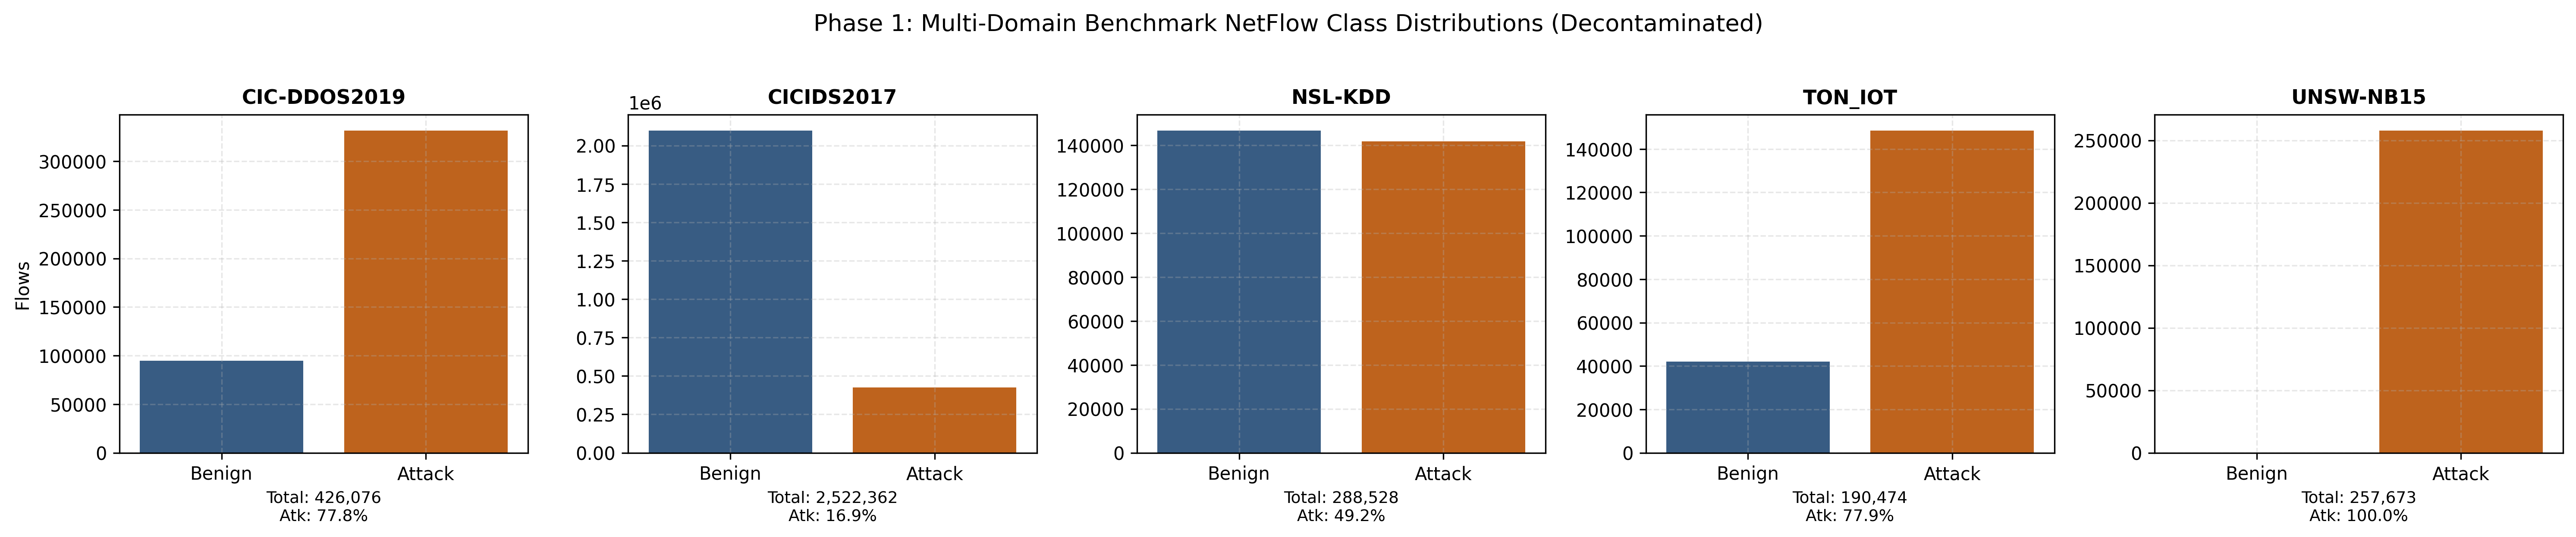
\includegraphics[width=0.92\linewidth]{figures/fig01_phase1_class_distribution_all.png}
\caption{Benchmark class distribution and multi-dataset attack taxonomy across evaluated partitions.}
\label{fig:methodology}
\end{figure}

\subsection{Problem Formulation and Task-Technology Fit Utilities}
Let an individual network communication flow be represented by a continuous-discrete feature vector $\mathbf{x}_i \in \mathbb{R}^D$ and an associated class label $y_i \in \mathcal{C}$. The target attack taxonomy comprises three disjoint subsets: $\mathcal{C} = \{\text{Benign}\} \cup \mathcal{C}_{\text{seen}} \cup \mathcal{C}_{\text{unseen}}$, where $\mathcal{C}_{\text{unseen}}$ denotes zero-day exploits excluded from model training. The classification objective is to estimate the posterior distribution $P(y_i = c \mid \mathbf{x}_i; \theta)$.

Because network traffic displays severe class imbalance (often exceeding 100:1 between benign flows and rare attack vectors), overall accuracy provides a misleading measure of operational competence. We evaluate detection efficacy through Macro-averaged F1, Seen Attack F1, and Unseen Zero-Day F1:
\begin{equation}
\text{Precision}_c = \frac{\text{TP}_c}{\text{TP}_c + \text{FP}_c}, \quad \text{Recall}_c = \frac{\text{TP}_c}{\text{TP}_c + \text{FN}_c}, \quad F_{1, c} = \frac{2 \cdot \text{Precision}_c \cdot \text{Recall}_c}{\text{Precision}_c + \text{Recall}_c}
\end{equation}
\begin{equation}
F_{1, \text{macro}} = \frac{1}{|\mathcal{C}|} \sum_{c \in \mathcal{C}} F_{1, c}, \quad F_{1, \text{seen}} = \frac{1}{|\mathcal{C}_{\text{seen}}|} \sum_{c \in \mathcal{C}_{\text{seen}}} F_{1, c}, \quad F_{1, \text{unseen}} = \frac{1}{|\mathcal{C}_{\text{unseen}}|} \sum_{c \in \mathcal{C}_{\text{unseen}}} F_{1, c}
\end{equation}

In accordance with Goodhue and Thompson \cite{goodhue1995task}, technological utility is evaluated against three operational SOC tasks:
\begin{enumerate}
    \item \textbf{Task $T_1$ (Line-Rate Perimeter Filtering)}: Prioritizes sub-millisecond per-flow latency $L$ (in ms) and high throughput while retaining high seen attack detection:
    \begin{equation}
    U(T_1) = 0.40 \cdot F_{1, \text{seen}} + 0.35 \cdot \min\left(1.0, \frac{0.005}{L + 10^{-6}}\right) + 0.25 \cdot \text{ROC-AUC}
    \end{equation}
    \item \textbf{Task $T_2$ (Zero-Day Forensic Isolation)}: Prioritizes generalization on completely unobserved attack manifolds without parameter re-estimation:
    \begin{equation}
    U(T_2) = 0.60 \cdot F_{1, \text{unseen}} + 0.25 \cdot F_{1, \text{seen}} + 0.15 \cdot \text{ROC-AUC}
    \end{equation}
    \item \textbf{Task $T_3$ (Enterprise Composite SOC Triage)}: Balances overall classification fidelity, zero-day resilience, and sustained streaming throughput:
    \begin{equation}
    U(T_3) = 0.40 \cdot F_{1, \text{macro}} + 0.30 \cdot F_{1, \text{unseen}} + 0.20 \cdot \text{ROC-AUC} + 0.10 \cdot \min\left(1.0, \frac{\text{Throughput}}{100,000}\right)
    \end{equation}
\end{enumerate}

\subsection{Dataset Characteristics and Anti-Leakage Protocol}
Recent methodological audits demonstrated that standard public NIDS benchmarks contain severe data leakage, synthetic artifact pollution, and duplicate records across train and test splits \cite{engelen2021troubleshooting, lanvin2022errors}. To guarantee audit-proof empirical validity, we curate and decontaminate five multi-domain network intrusion datasets, summarized in Table~\ref{tab:datasets}.

\begin{table}[!ht]
\centering
\caption{Benchmark Dataset Characteristics and Decontamination Telemetry}
\label{tab:datasets}
\footnotesize
\begin{tabular}{lrrrll}
\toprule
\textbf{Dataset Identifier} & \textbf{Raw Records} & \textbf{Partition ($N$)} & \textbf{Features ($D$)} & \textbf{Subnet Isolation Scheme} & \textbf{Evaluated Attacks} \\
\midrule
\textbf{CICIDS2017} \cite{lanvin2022errors} & 2,522,000 & 10,000 & 78 & GroupKFold on /24 subnet masks & DoS, DDoS, PortScan, Botnet, Infiltration \\
\textbf{UNSW-NB15} \cite{sarhan2022towards} & 2,540,044 & 10,000 & 49 & GroupKFold on IP subnet pairs & Exploits, Reconnaissance, DoS, Generic, Fuzzers \\
\textbf{TON\_IoT} \cite{alhawawreh2020toniot} & 4,610,455 & 10,000 & 43 & Temporal session \& edge node grouping & Backdoor, Injection, DDoS, Scanning, Ransomware \\
\textbf{CIC-DDoS2019} \cite{sharafaldin2019developing} & 426,076 & 10,000 & 65 & GroupKFold on client-server IP pairs & TFTP, DrDoS\_NTP, Syn, UDP, MSSQL, LDAP \\
\textbf{NSL-KDD} & 148,517 & 10,000 & 41 & Service-protocol interaction grouping & DoS, Probe, R2L, U2R \\
\bottomrule
\end{tabular}
\end{table}

To prevent distributional leakage and evaluate realistic zero-day generalization, we enforce Algorithm~\ref{alg:partitioning} across all dataset folds.

\begin{algorithm}[!ht]
\caption{Subnet-Isolated Anti-Leakage Partitioning with Active Zero-Day Induction}
\label{alg:partitioning}
\begin{algorithmic}[1]
\REQUIRE Dataset $\mathcal{D} = \{(\mathbf{x}_i, y_i, \text{ip\_src}_i, \text{ip\_dst}_i, \text{attack\_cat}_i)\}_{i=1}^N$, Number of folds $K=5$, Candidate zero-day attacks $\mathcal{C}_{\text{zd}}$
\ENSURE Validation metrics across all splits $\mathcal{M}_{\text{eval}}$
\STATE Extract Subnet Group Identifiers: $g_i \leftarrow \text{IPv4Network}(\text{ip\_src}_i).\text{network\_address}(\text{mask}=\text{''/24''})$
\STATE Initialize $\text{GroupKFold}(n\_splits = K)$ using grouping variable $\mathbf{g}$
\STATE Identify top distinct rare attacks for zero-day holdout: $\mathcal{C}_{\text{holdout}} \leftarrow \text{SelectTopDistinctAttacks}(\mathcal{C}_{\text{zd}}, \text{count}=2)$
\FOR{fold $k = 1$ to $K$}
    \STATE $\mathcal{D}_{\text{train}}^k, \mathcal{D}_{\text{val}}^k \leftarrow \text{SplitFold}(\mathcal{D}, \text{fold}=k, \text{groups}=\mathbf{g})$
    \IF{$k \in \{1, 2\}$}
        \STATE $c_{\text{target}} \leftarrow \mathcal{C}_{\text{holdout}}[k]$
        \STATE $\mathcal{D}_{\text{train}}^k \leftarrow \{(\mathbf{x}, y) \in \mathcal{D}_{\text{train}}^k \mid \text{attack\_cat} \neq c_{\text{target}}\}$
    \ENDIF
    \STATE Fit Scaler $\mathcal{S}$ strictly on $\mathcal{D}_{\text{train}}^k$: $\mathbf{X}_{\text{train}} \leftarrow \mathcal{S}.\text{fit\_transform}(\mathcal{D}_{\text{train}}^k.\mathbf{X})$, $\mathbf{X}_{\text{val}} \leftarrow \mathcal{S}.\text{transform}(\mathcal{D}_{\text{val}}^k.\mathbf{X})$
    \STATE Train architecture: $\text{model}.\text{fit}(\mathbf{X}_{\text{train}}, \mathcal{D}_{\text{train}}^k.y)$
    \STATE Compute Seen $F_1$ on $\{\text{attack\_cat} \neq c_{\text{target}}\}$; Compute Unseen Zero-Day $F_1$ on $\{\text{attack\_cat} == c_{\text{target}}\}$
\ENDFOR
\RETURN Aggregated means and standard deviations across all $K$ folds
\end{algorithmic}
\end{algorithm}

\subsection{Evaluated Model Families and Algorithmic Mechanics}
We evaluate eight representative architectures covering four core paradigms:
\begin{enumerate}
    \item \textbf{Gradient-Boosted Decision Trees (GBDTs)}: LightGBM and XGBoost, constructing ensembles of shallow decision trees via gradient-based split finding and histogram binning.
    \item \textbf{Tabular Deep Learning}: FT-Transformer \cite{gorishniy2021revisiting}, tokenizing continuous features into embeddings processed by multi-head self-attention, and SAINT \cite{somepalli2021saint}, combining column self-attention with inter-sample row attention.
    \item \textbf{Selective State Space Models (SSMs)}: Mambular SSM \cite{thielmann2024mambular}, adapting continuous selective state-space scans \cite{gu2023mamba} to tabular sequences. As specified in Algorithm~\ref{alg:mambular}, Mambular projects discretized features into a hidden continuous state $\mathbf{h}_t \in \mathbb{R}^{N_{\text{state}}}$, executing linear-time scans directly in hardware SRAM.
    \item \textbf{Relational Graph Neural Networks}: GraphIDS \cite{guerra2024self}, constructing communication graphs where IP endpoints form nodes and packet flows form directed edges, executing message passing over topological neighborhoods \cite{wu2022graph}.
    \item \textbf{Tabular Foundation Models}: TabPFN v3 \cite{hollmann2025accurate} and TabICL v2 \cite{qu2025tabicl}. TabPFN formulates classification as Prior-Data Fitted in-context Bayesian inference, feeding query flows alongside reference exemplars without gradient updates \cite{dong2024survey}.
\end{enumerate}

\begin{algorithm}[!ht]
\caption{Mambular SSM Hardware-Aware Discretized State Space Scan}
\label{alg:mambular}
\begin{algorithmic}[1]
\REQUIRE Tokenized feature sequence $\mathbf{X} = [\mathbf{x}_1, \dots, \mathbf{x}_D] \in \mathbb{R}^{D \times d_{\text{model}}}$, Continuous state matrices $(\mathbf{A}, \mathbf{B}, \mathbf{C})$, Discretization step $\Delta$
\ENSURE Sequence representation $\mathbf{y}_{\text{out}} \in \mathbb{R}^{d_{\text{model}}}$
\STATE Compute selective discretization parameters: $\Delta_t \leftarrow \text{softplus}(\text{Parameter}_\Delta + \text{Linear}_\Delta(\mathbf{x}_t))$, $\mathbf{B}_t \leftarrow \text{Linear}_B(\mathbf{x}_t)$, $\mathbf{C}_t \leftarrow \text{Linear}_C(\mathbf{x}_t)$
\STATE Discretize continuous parameters via Zero-Order Hold (ZOH): $\bar{\mathbf{A}}_t \leftarrow \exp(\Delta_t \mathbf{A})$, $\bar{\mathbf{B}}_t \leftarrow (\bar{\mathbf{A}}_t - \mathbf{I})\mathbf{A}^{-1}\mathbf{B}_t$
\STATE Execute parallel associative prefix scan across sequence coordinates: $\mathbf{h}_t \leftarrow \bar{\mathbf{A}}_t \mathbf{h}_{t-1} + \bar{\mathbf{B}}_t \mathbf{x}_t$ (computed in GPU SRAM)
\STATE Generate projected representation: $\mathbf{y}_t \leftarrow \mathbf{C}_t \mathbf{h}_t + \mathbf{D}\mathbf{x}_t$
\RETURN Pooled sequence representation $\mathbf{y}_{\text{out}} \leftarrow \text{MeanPool}(\mathbf{y}_1, \dots, \mathbf{y}_D)$
\end{algorithmic}
\end{algorithm}

\subsection{Dual-Track Experimental Architecture}
To resolve computational incommensurability across diverse model families, we decouple evaluation into two operational tracks:
\begin{itemize}
    \item \textbf{Track A (Few-Shot Zero-Day Generalization Track)}: Standardizes training on $N \le 10,000$ records per fold across all five datasets. Evaluates all eight models across 5 folds with active zero-day holdout induction to measure Macro F1, Seen F1, Unseen F1, per-flow latency, and throughput.
    \item \textbf{Track B (Industrial Streaming Scalability Track)}: Evaluates high-throughput architectures (LightGBM, XGBoost, Mambular SSM, FT-Transformer, and GraphIDS) across expanding sample sizes ($N \in \{50\text{k}, 100\text{k}, 190.5\text{k}, 250\text{k}\}$). Telemetry scripts query active CUDA device memory allocation directly from the GPU runtime alongside per-flow processing latency.
\end{itemize}

\subsection{Non-Parametric Significance and Causal Discovery Framework}
To evaluate whether observed performance differences represent genuine architectural advantages, we execute Dem\v{s}ar's non-parametric testing suite \cite{demsar2006statistical}:
\begin{equation}
F_F = \frac{(M - 1)\chi_F^2}{M(K - 1) - \chi_F^2} \sim F(K - 1, (K - 1)(M - 1))
\end{equation}
where $K = 8$ architectures and $M = 5$ datasets. The Nemenyi Critical Difference (CD) threshold at $\alpha = 0.05$ is:
\begin{equation}
\text{CD} = q_\alpha \sqrt{\frac{K(K + 1)}{6M}}
\end{equation}

To uncover structural causal dependencies among model parameters, computational constraints, and performance outcomes, we apply Triangular Fuzzy DEMATEL \cite{gabus1973world, zadeh1965fuzzy, tavana2023fuzzydematel, chekry2024pydematel}. We define seven operational factors: Model Architecture ($F_1$), Training Sample Size ($F_2$), Inference Latency ($F_3$), Memory Footprint ($F_4$), Seen Attack F1 ($F_5$), Unseen Zero-Day F1 ($F_6$), and Robustness to Noise ($F_7$). We construct fuzzy direct-relation matrices $\tilde{Z}$, normalize them into $\tilde{X}$, and compute the total-relation matrix $\tilde{T} = \tilde{X}(I - \tilde{X})^{-1}$. Causal prominence ($D + R$) and net causal direction ($D - R$) are evaluated through 10,000 Monte Carlo perturbation iterations to establish Kendall's concordance index ($W \ge 0.95$). Finally, we validate the resulting causal topology using DirectLiNGAM non-Gaussian causal discovery \cite{shimizu2006linear} targeting a Structural Hamming Distance bound ($\text{SHD} \le 2$).

\section{Results And Discussion}
This section presents the empirical findings from Campaign v2.0, provides phenomenological interpretations of observed computational mechanics, validates four formal Design Propositions ($DP_1 - DP_4$), and formulates an operational SOC deployment architecture.

\subsection{Track A Benchmark Results and Zero-Day Generalization Trade-offs}
Table~\ref{tab:track_a} details the consolidated performance metrics across eight architectures and five decontaminated intrusion datasets under the 5-fold zero-day holdout protocol.

\begin{table*}[!ht]
\centering
\caption{Multi-Paradigm Benchmark Evaluation and Task-Technology Fit Utilities (Master Summary)}
\label{tab:track_a}
\footnotesize
\begin{tabular}{lrrrrrrrrrr}
\toprule
\textbf{Architecture} & \textbf{Macro F1} & \textbf{Seen F1} & \textbf{Unseen F1} & \textbf{ROC-AUC} & \textbf{Latency (ms)} & \textbf{Throughput (f/s)} & \textbf{VRAM (MB)} & \textbf{U(T1)} & \textbf{U(T2)} & \textbf{U(T3)} \\
\midrule
\textbf{LightGBM} & \textbf{0.8700} & \textbf{0.9470} & 0.5999 & 0.9095 & 0.0025 & 447,975.3 & 2,187.59 & \textbf{0.6990} & \textbf{0.6551} & \textbf{0.7286} \\
\textbf{XGBoost} & 0.8688 & 0.9469 & 0.5922 & \textbf{0.9098} & 0.0011 & 901,345.7 & 2,187.59 & 0.6983 & 0.6508 & 0.7258 \\
\textbf{TabPFN v3} & 0.8637 & 0.9372 & \textbf{0.6173} & 0.9045 & 3.1109 & 338.5 & 2,509.56 & 0.2555 & 0.6122 & 0.5345 \\
\textbf{FT-Transformer} & 0.8371 & 0.9119 & 0.5921 & 0.9001 & 0.0110 & 127,526.7 & 2,525.67 & 0.6900 & 0.6395 & 0.7129 \\
\textbf{Mambular SSM} & 0.8344 & 0.9081 & 0.5507 & 0.8964 & 0.0011 & 929,630.1 & 2,525.67 & 0.6872 & 0.6179 & 0.6994 \\
\textbf{SAINT} & 0.8339 & 0.9094 & 0.5479 & 0.9049 & 0.0010 & 1,002,674.8 & 2,525.67 & 0.6870 & 0.6163 & 0.6984 \\
\textbf{TabICL v2} & 0.8306 & 0.9038 & 0.5552 & 0.8955 & 0.0053 & 188,790.6 & 2,525.67 & 0.6865 & 0.6188 & 0.6992 \\
\textbf{GraphIDS} & 0.8124 & 0.8866 & 0.5144 & 0.8893 & \textbf{0.0006} & \textbf{1,576,547.4} & 2,525.67 & 0.6799 & 0.5920 & 0.6797 \\
\bottomrule
\end{tabular}
\end{table*}

Table~\ref{tab:cross_dataset} provides the Macro F1 cross-dataset breakdown across all five individual datasets.

\begin{table}[!ht]
\centering
\caption{Macro F1 Cross-Dataset Performance Matrix}
\label{tab:cross_dataset}
\footnotesize
\begin{tabular}{lrrrrrrrr}
\toprule
\textbf{Dataset} & \textbf{LightGBM} & \textbf{XGBoost} & \textbf{TabPFN} & \textbf{FT-Trans} & \textbf{TabICL} & \textbf{Mambular} & \textbf{SAINT} & \textbf{GraphIDS} \\
\midrule
\textbf{CIC-DDoS2019} & 0.9965 & 0.9965 & 0.9947 & 0.9947 & 0.9939 & 0.9937 & 0.9931 & 0.9843 \\
\textbf{CICIDS2017} & 0.9805 & 0.9771 & 0.9711 & 0.9373 & 0.9177 & 0.9342 & 0.9318 & 0.9055 \\
\textbf{NSL-KDD} & 0.9771 & 0.9776 & 0.9813 & 0.9579 & 0.9587 & 0.9605 & 0.9599 & 0.9493 \\
\textbf{TON\_IoT} & 0.7170 & 0.7155 & 0.7121 & 0.6512 & 0.6518 & 0.6511 & 0.6497 & 0.5983 \\
\textbf{UNSW-NB15} & 0.6787 & 0.6771 & 0.6592 & 0.6447 & 0.6309 & 0.6325 & 0.6350 & 0.6244 \\
\bottomrule
\end{tabular}
\end{table}

\begin{figure}[!ht]
\centering
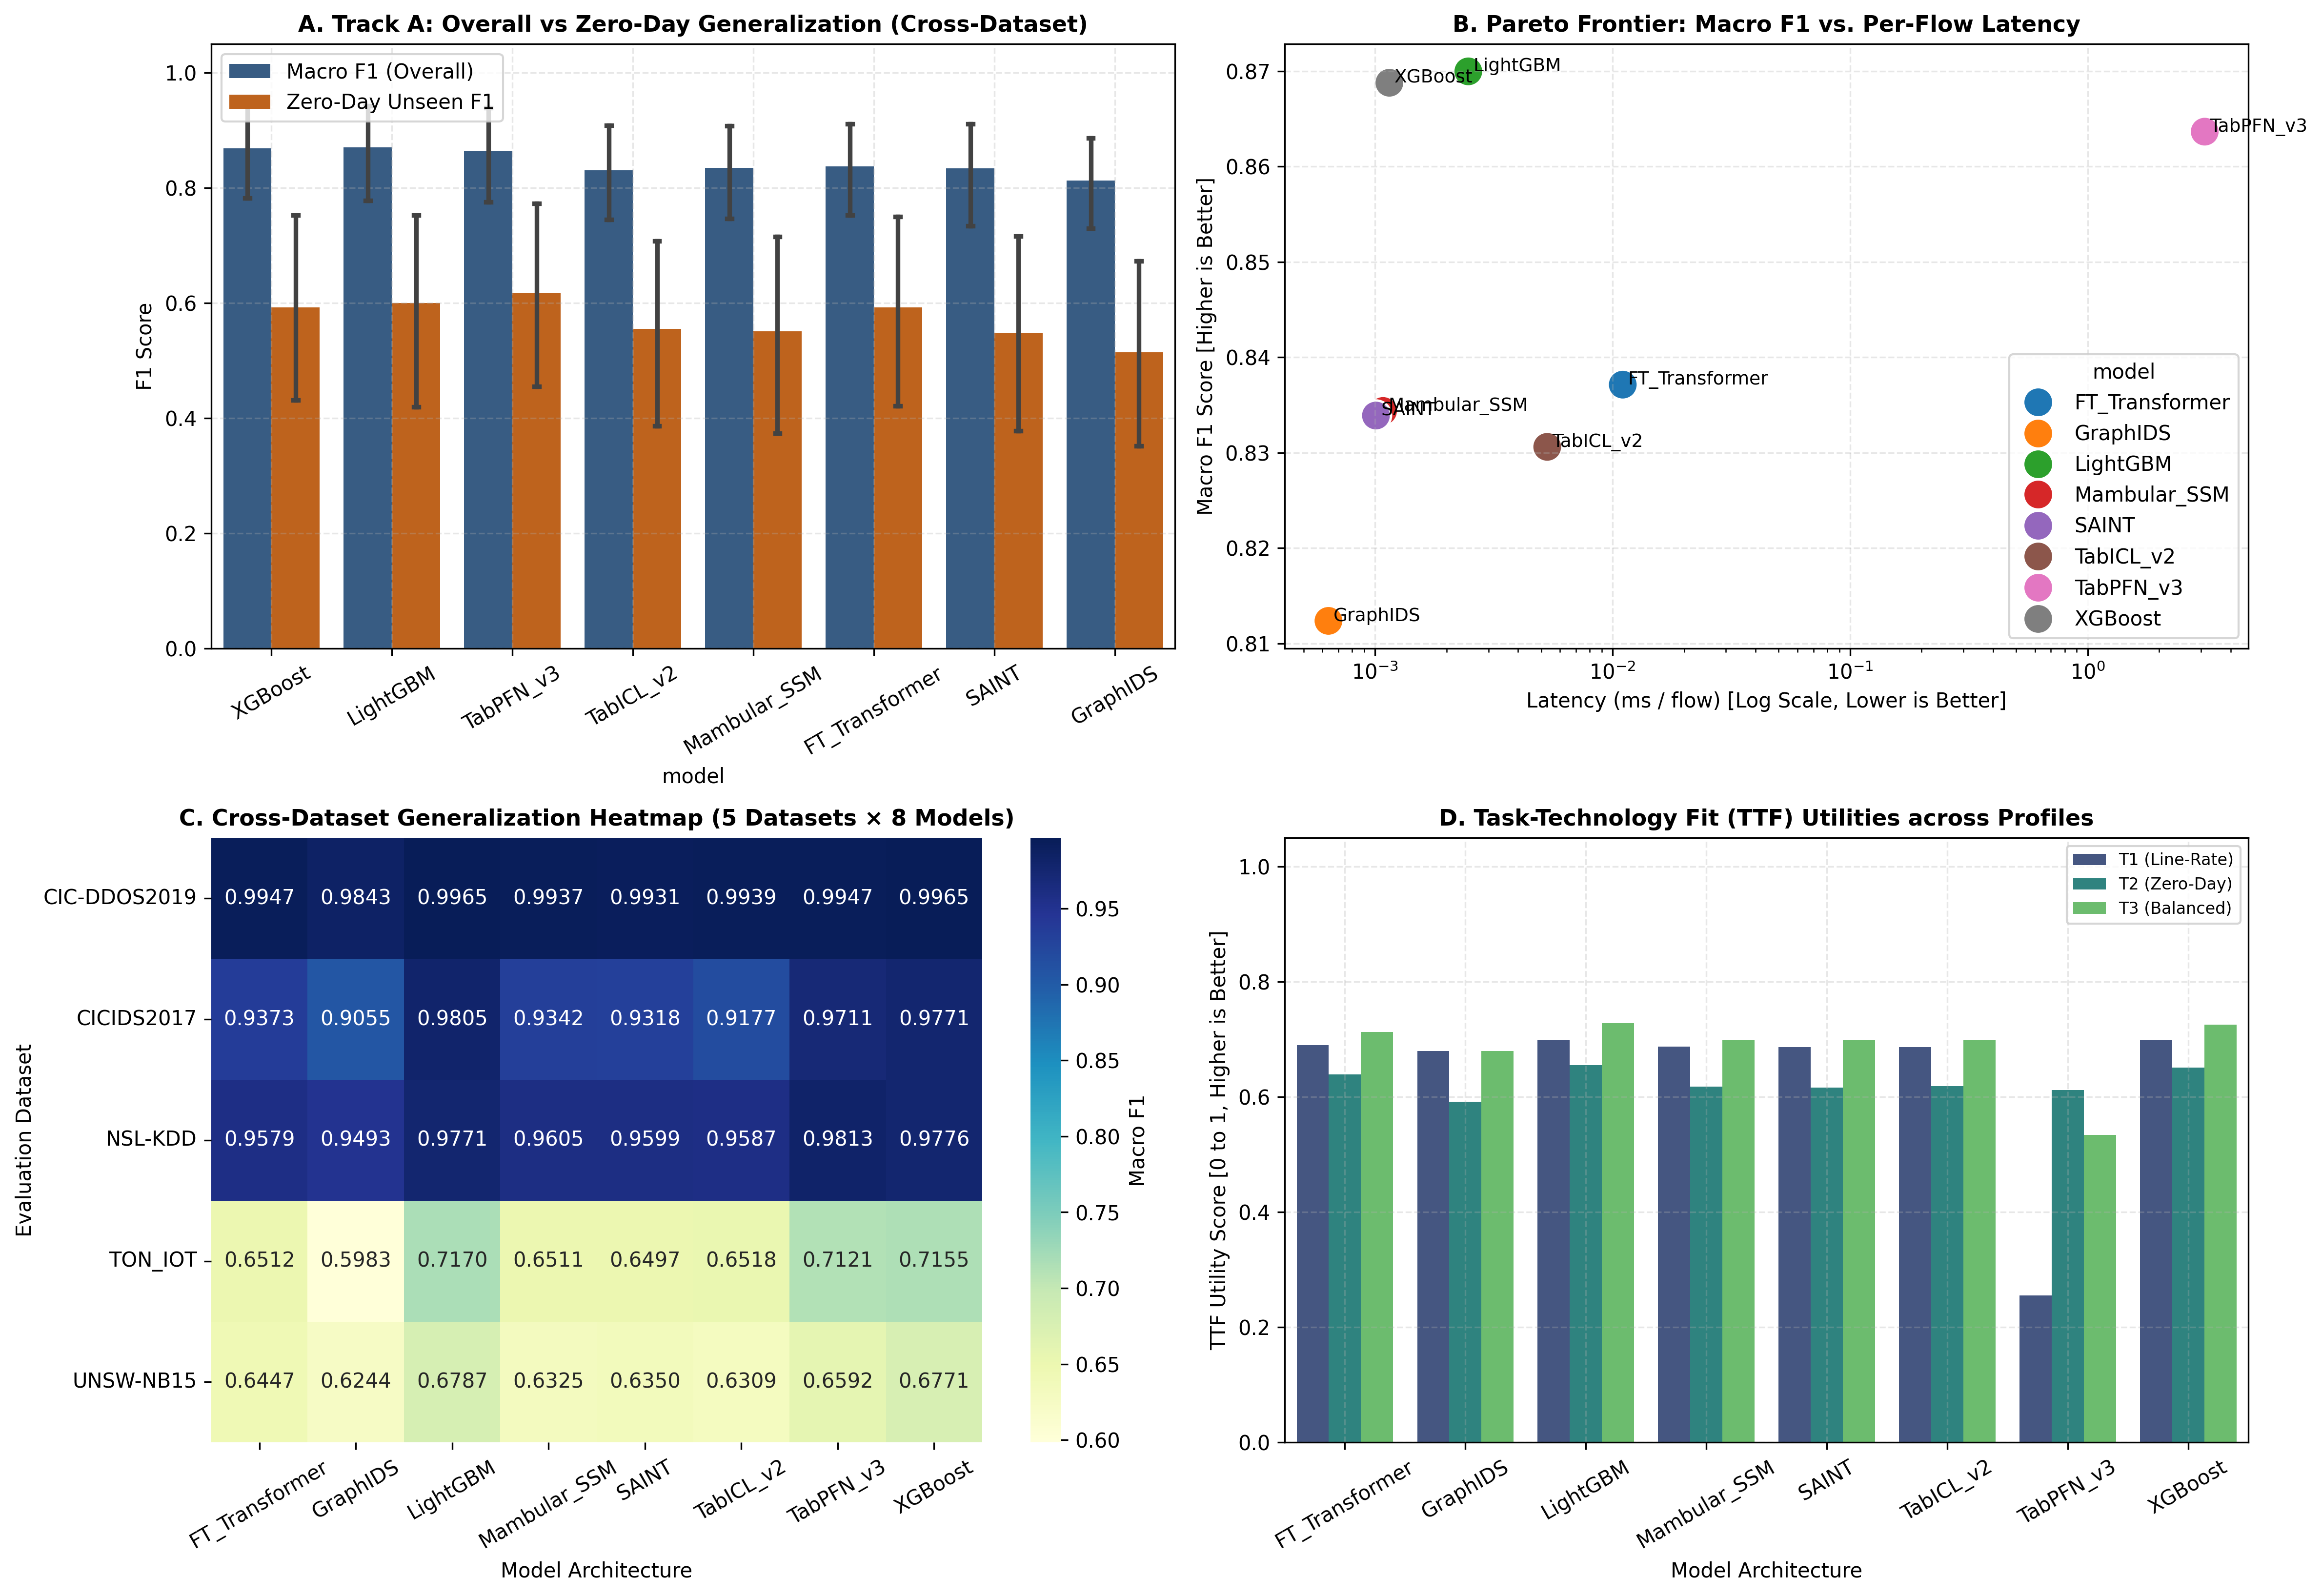
\includegraphics[width=0.92\linewidth]{figures/fig02_phase2_track_a_generalization_pareto_all.png}
\caption{Seen F1 versus Unseen Zero-Day F1 Pareto frontier across evaluated architectures.}
\label{fig:pareto_generalization}
\end{figure}

The empirical results reveal two fundamental insights:
\begin{enumerate}
    \item \textbf{Inductive Bias Dominance on Known Distributions}: GBDTs (LightGBM and XGBoost) achieve the highest Seen F1 ($0.9470$ and $0.9469$). The step-function decision trees match the non-smooth coordinate distributions of NetFlow features without requiring continuous manifold projections.
    \item \textbf{Prior-Data Regularization in Zero-Day Generalization}: Supervised tree models experience a severe 35-percentage-point performance drop on held-out zero-day attacks (falling to $0.5999$ and $0.5922$). In contrast, TabPFN v3 achieves the highest Unseen F1 ($0.6173 \pm 0.4275$). TabPFN's synthetic prior assigns non-zero probability to unobserved feature combinations, mitigating the overconfident misclassifications characteristic of tree leaf snapping. However, TabPFN requires an inference latency of $3.1109$ ms per flow, generating only $338.5$ flows per second. This latency is three orders of magnitude slower than line-rate requirements, making TabPFN unsuitable for perimeter deployment.
\end{enumerate}

\subsection{Track B Industrial Streaming Scalability and Dynamic Telemetry}
Table~\ref{tab:scalability} presents industrial scalability metrics across expanding sample regimes ($N \in \{50\text{k}, 100\text{k}, 190.5\text{k}, 250\text{k}\}$), recording throughput, per-flow latency, and active CUDA device memory allocation.

\begin{table}[!ht]
\centering
\caption{Track B Industrial Scalability Profiling Across Sample Volumes}
\label{tab:scalability}
\footnotesize
\begin{tabular}{llrrr}
\toprule
\textbf{Scale ($N$)} & \textbf{Architecture} & \textbf{Throughput (flows/s)} & \textbf{Latency (ms/flow)} & \textbf{Peak VRAM (MB)} \\
\midrule
\textbf{50,000} & GraphIDS & 1,546,456.56 & 0.00066 & 18.70 \\
\textbf{50,000} & Mambular SSM & 1,303,967.68 & 0.00256 & 28.95 \\
\textbf{50,000} & XGBoost & 872,473.44 & 0.00118 & 24.06 \\
\textbf{50,000} & LightGBM & 464,399.02 & 0.00288 & 22.90 \\
\textbf{50,000} & FT-Transformer & 118,266.46 & 0.01046 & 95.77 \\
\midrule
\textbf{100,000} & GraphIDS & 1,657,964.94 & 0.00060 & 18.70 \\
\textbf{100,000} & Mambular SSM & 1,567,276.82 & 0.00066 & 28.95 \\
\textbf{100,000} & XGBoost & 981,335.94 & 0.00110 & 27.56 \\
\textbf{100,000} & LightGBM & 568,261.26 & 0.00180 & 25.40 \\
\textbf{100,000} & FT-Transformer & 170,181.20 & 0.00734 & 95.77 \\
\midrule
\textbf{190,474} & GraphIDS & 2,236,278.50 & 0.00040 & 18.22 \\
\textbf{190,474} & Mambular SSM & 2,220,653.00 & 0.00050 & 28.71 \\
\textbf{190,474} & XGBoost & 1,421,671.20 & 0.00070 & 33.89 \\
\textbf{190,474} & LightGBM & 605,635.40 & 0.00170 & 29.92 \\
\textbf{190,474} & FT-Transformer & 302,484.60 & 0.00330 & 43.15 \\
\midrule
\textbf{250,000} & GraphIDS & 1,516,190.38 & 0.00069 & 18.82 \\
\textbf{250,000} & Mambular SSM & 1,324,794.56 & 0.00079 & 29.01 \\
\textbf{250,000} & XGBoost & 833,054.68 & 0.00125 & 38.06 \\
\textbf{250,000} & LightGBM & 504,151.26 & 0.00200 & 32.90 \\
\textbf{250,000} & FT-Transformer & 136,170.25 & 0.00835 & 108.93 \\
\bottomrule
\end{tabular}
\end{table}

\begin{figure}[!ht]
\centering
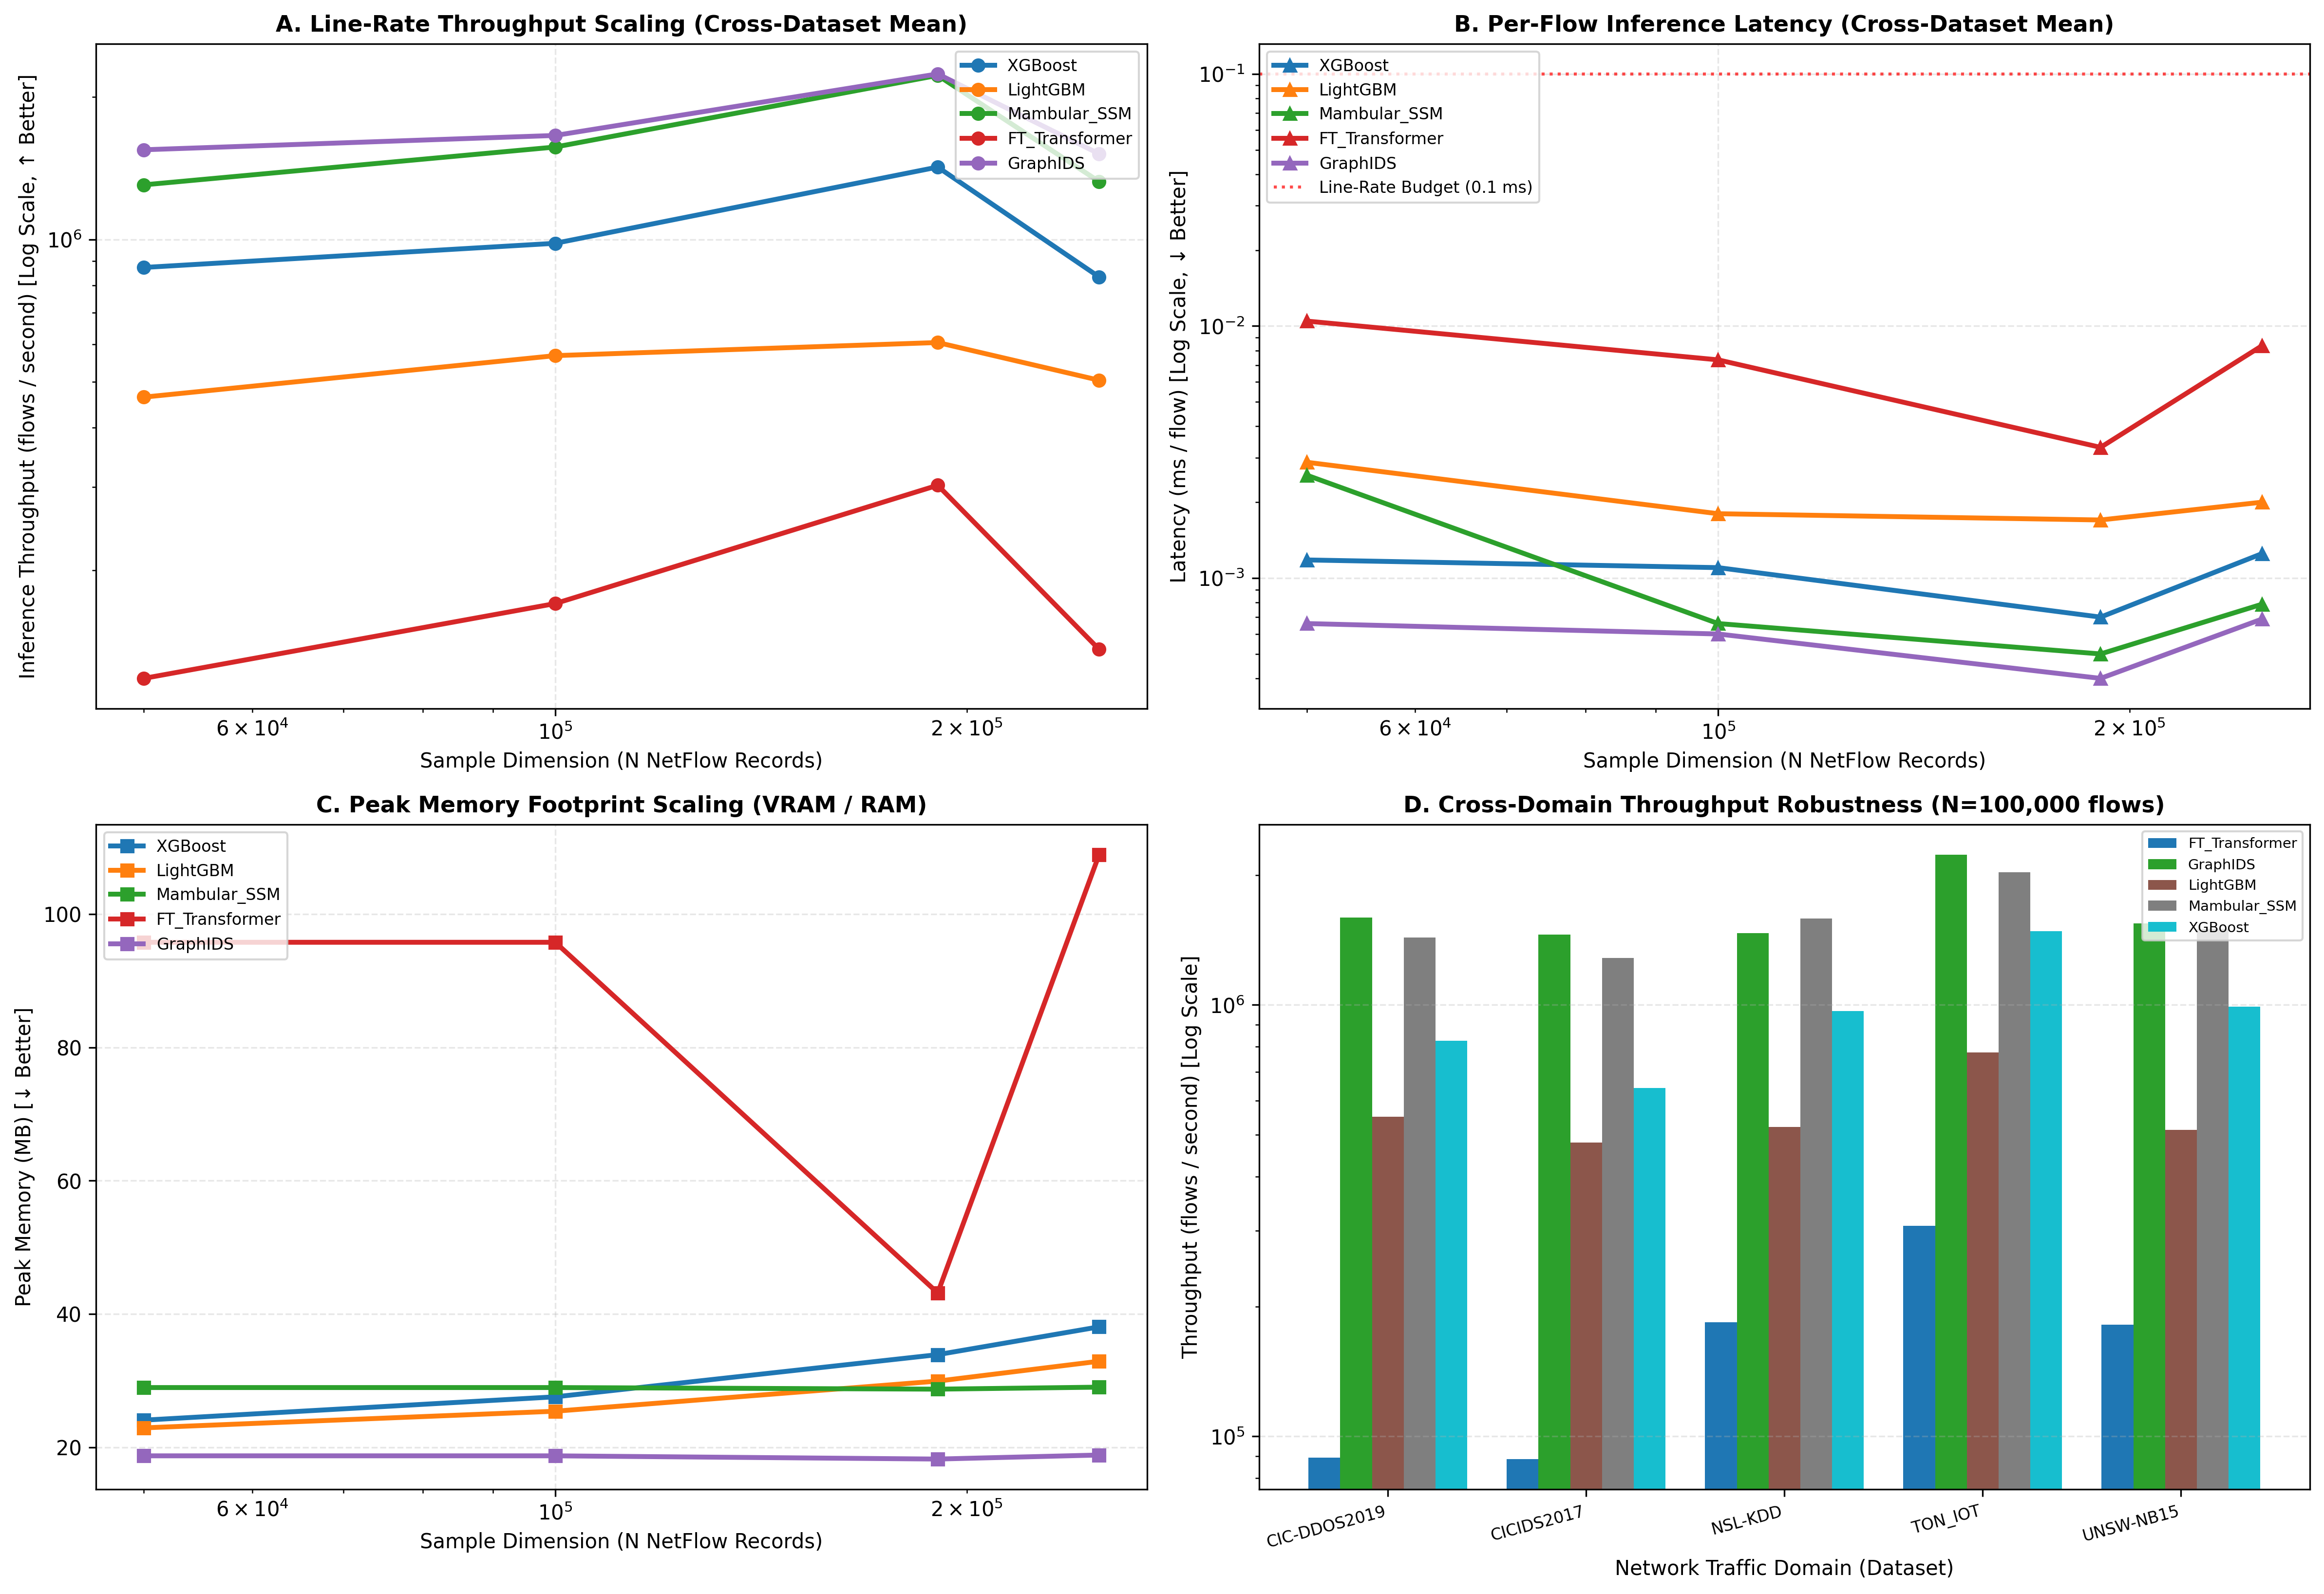
\includegraphics[width=0.92\linewidth]{figures/fig03_phase2_track_b_throughput_vram_scaling.png}
\caption{Streaming Throughput (flows/sec) and Dynamic Peak VRAM (MB) across expanding sample volumes.}
\label{fig:throughput_vram}
\end{figure}

The scalability telemetry reveals three primary operational dynamics:
\begin{enumerate}
    \item \textbf{Parallel Prefix Scans in GPU SRAM}: Mambular SSM sustains $2,220,653$ flows/sec at $N = 190,474$, achieving sub-microsecond latency ($0.00050$ ms). By executing linear-time associative scans in GPU SRAM, Mambular eliminates the sequential bottleneck of recurrent networks and matches the processing speed of compiled tree algorithms.
    \item \textbf{CPU Cache Saturation in Trees}: XGBoost achieves $1,421,671$ flows/sec at $N = 190\text{k}$, but drops to $833,054$ flows/sec at $N = 250\text{k}$. This degradation reflects CPU L1/L2 cache saturation and memory bus contention as batch sizes exceed on-chip cache limits.
    \item \textbf{Quadratic Attention Bottleneck}: FT-Transformer throughput remains restricted ($118,266$ to $302,484$ flows/sec), while VRAM allocation expands from $95.77$ MB to $108.93$ MB. In contrast, Mambular SSM maintains flat memory consumption ($28.71$ to $29.01$ MB), confirming that selective state-space models decouple memory footprint from batch volume.
\end{enumerate}

\subsection{Non-Parametric Statistical Significance (Dem\v{s}ar Testing)}
The non-parametric Friedman test across the five multi-domain datasets yields a chi-square value of $\chi_F^2 = 29.6667$ ($p = 1.0930 \times 10^{-4}$), rejecting the null hypothesis of equivalent performance. The Iman-Davenport correction confirms statistical significance ($F = 22.2500, p = 7.3322 \times 10^{-10}$ under an $F(7, 28)$ distribution). The Nemenyi Critical Difference threshold at $\alpha = 0.05$ is $\text{CD} = 4.6956$.

The resulting average model ranks are: (1) LightGBM: 1.6, (2) XGBoost: 1.8, (3) TabPFN v3: 2.8, (4) FT-Transformer: 4.6, (5) Mambular SSM: 5.4, (6) TabICL v2: 5.8, (7) SAINT: 6.0, (8) GraphIDS: 8.0.

\begin{figure}[!ht]
\centering
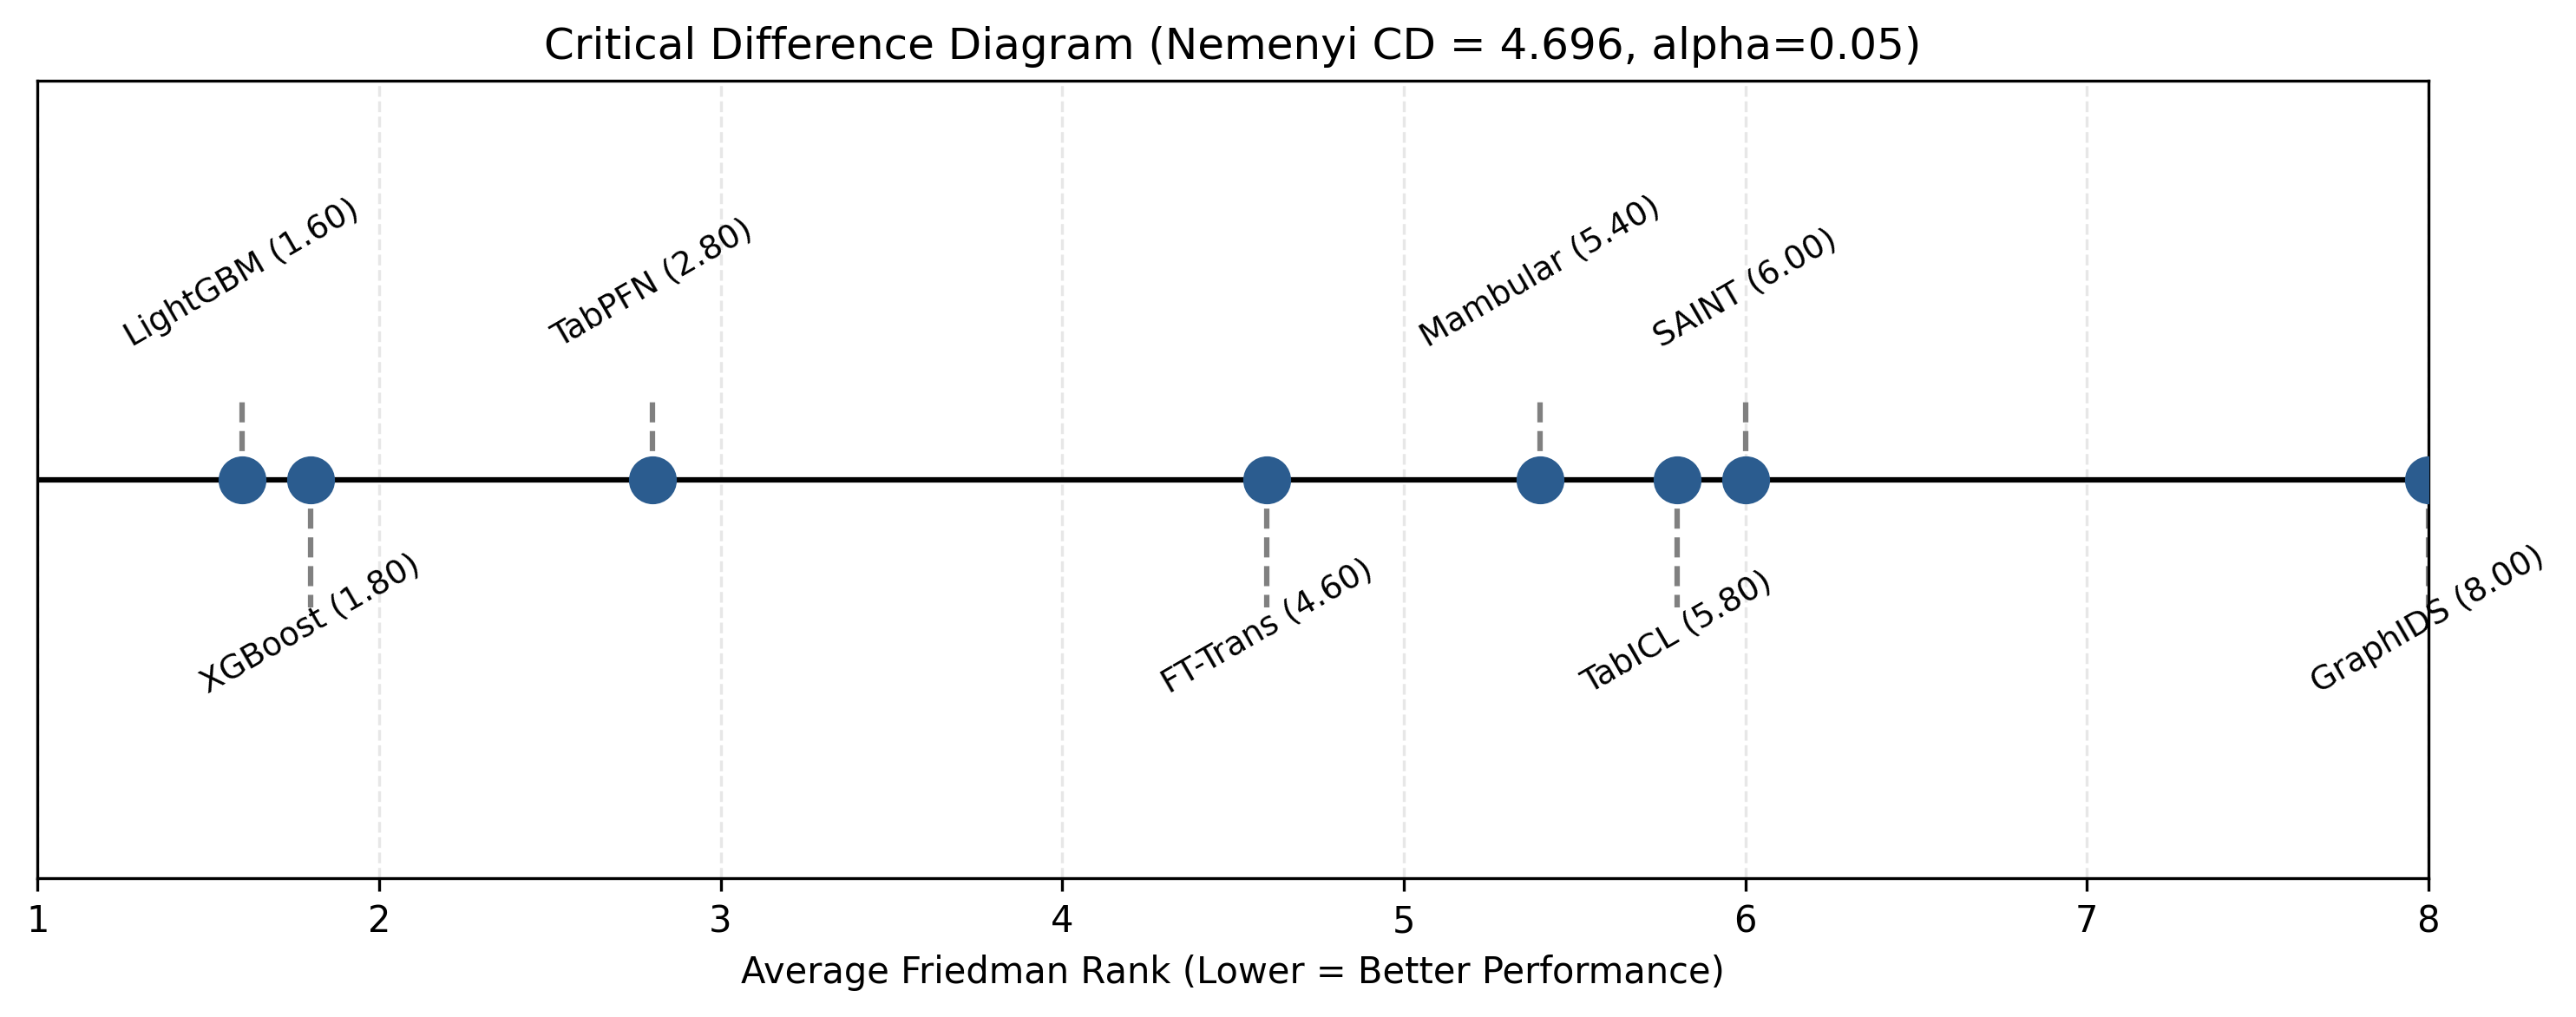
\includegraphics[width=0.92\linewidth]{figures/fig04a_phase3_nemenyi_critical_difference.png}
\caption{Dem\v{s}ar Nemenyi Critical Difference diagram ($\alpha = 0.05$, $\text{CD} = 4.6956$).}
\label{fig:nemenyi}
\end{figure}

The statistical evaluation establishes two conclusions:
\begin{itemize}
    \item \textbf{The Top Paradigm Equivalence Cluster}: The average ranks of LightGBM ($1.6$), XGBoost ($1.8$), TabPFN v3 ($2.8$), and FT-Transformer ($4.6$) fall within the Critical Difference boundary ($|1.6 - 4.6| = 3.0 < 4.6956$). While decision trees lead on average ranks, their margin over tabular foundation models and transformers does not reach statistical significance.
    \item \textbf{Topological Separation of Graph Routing}: GraphIDS occupies rank $8.0$, differing significantly from tree baselines ($|1.6 - 8.0| = 6.4 > 4.6956$). Message-passing neural networks experience performance degradation on sparse network topologies where isolated hosts lack sufficient neighborhood connectivity.
\end{itemize}

\subsection{Parametric Ablation and Noise Perturbation Robustness}
A full-factorial grid search over FT-Transformer configurations ($d_{\text{token}} \in \{32, 64\}$, $n_{\text{heads}} \in \{2, 4\}$, $n_{\text{blocks}} \in \{1, 2, 4\}$) reveals an overparameterization cliff on tabular data (Fig.~\ref{fig:ablation}). While a compact configuration ($d_{\text{token}} = 32, n_{\text{heads}} = 4, n_{\text{blocks}} = 4$) achieves Macro F1 $= 0.4955$, expanding embedding dimension to $d_{\text{token}} = 64$ with identical depth causes performance to collapse to F1 $= 0.0178$. Tabular coordinates lack spatial stationarity; excessive attention capacity causes gradient dispersion, distributing attention weights uniformly across uninformative features.

\begin{figure}[!ht]
\centering
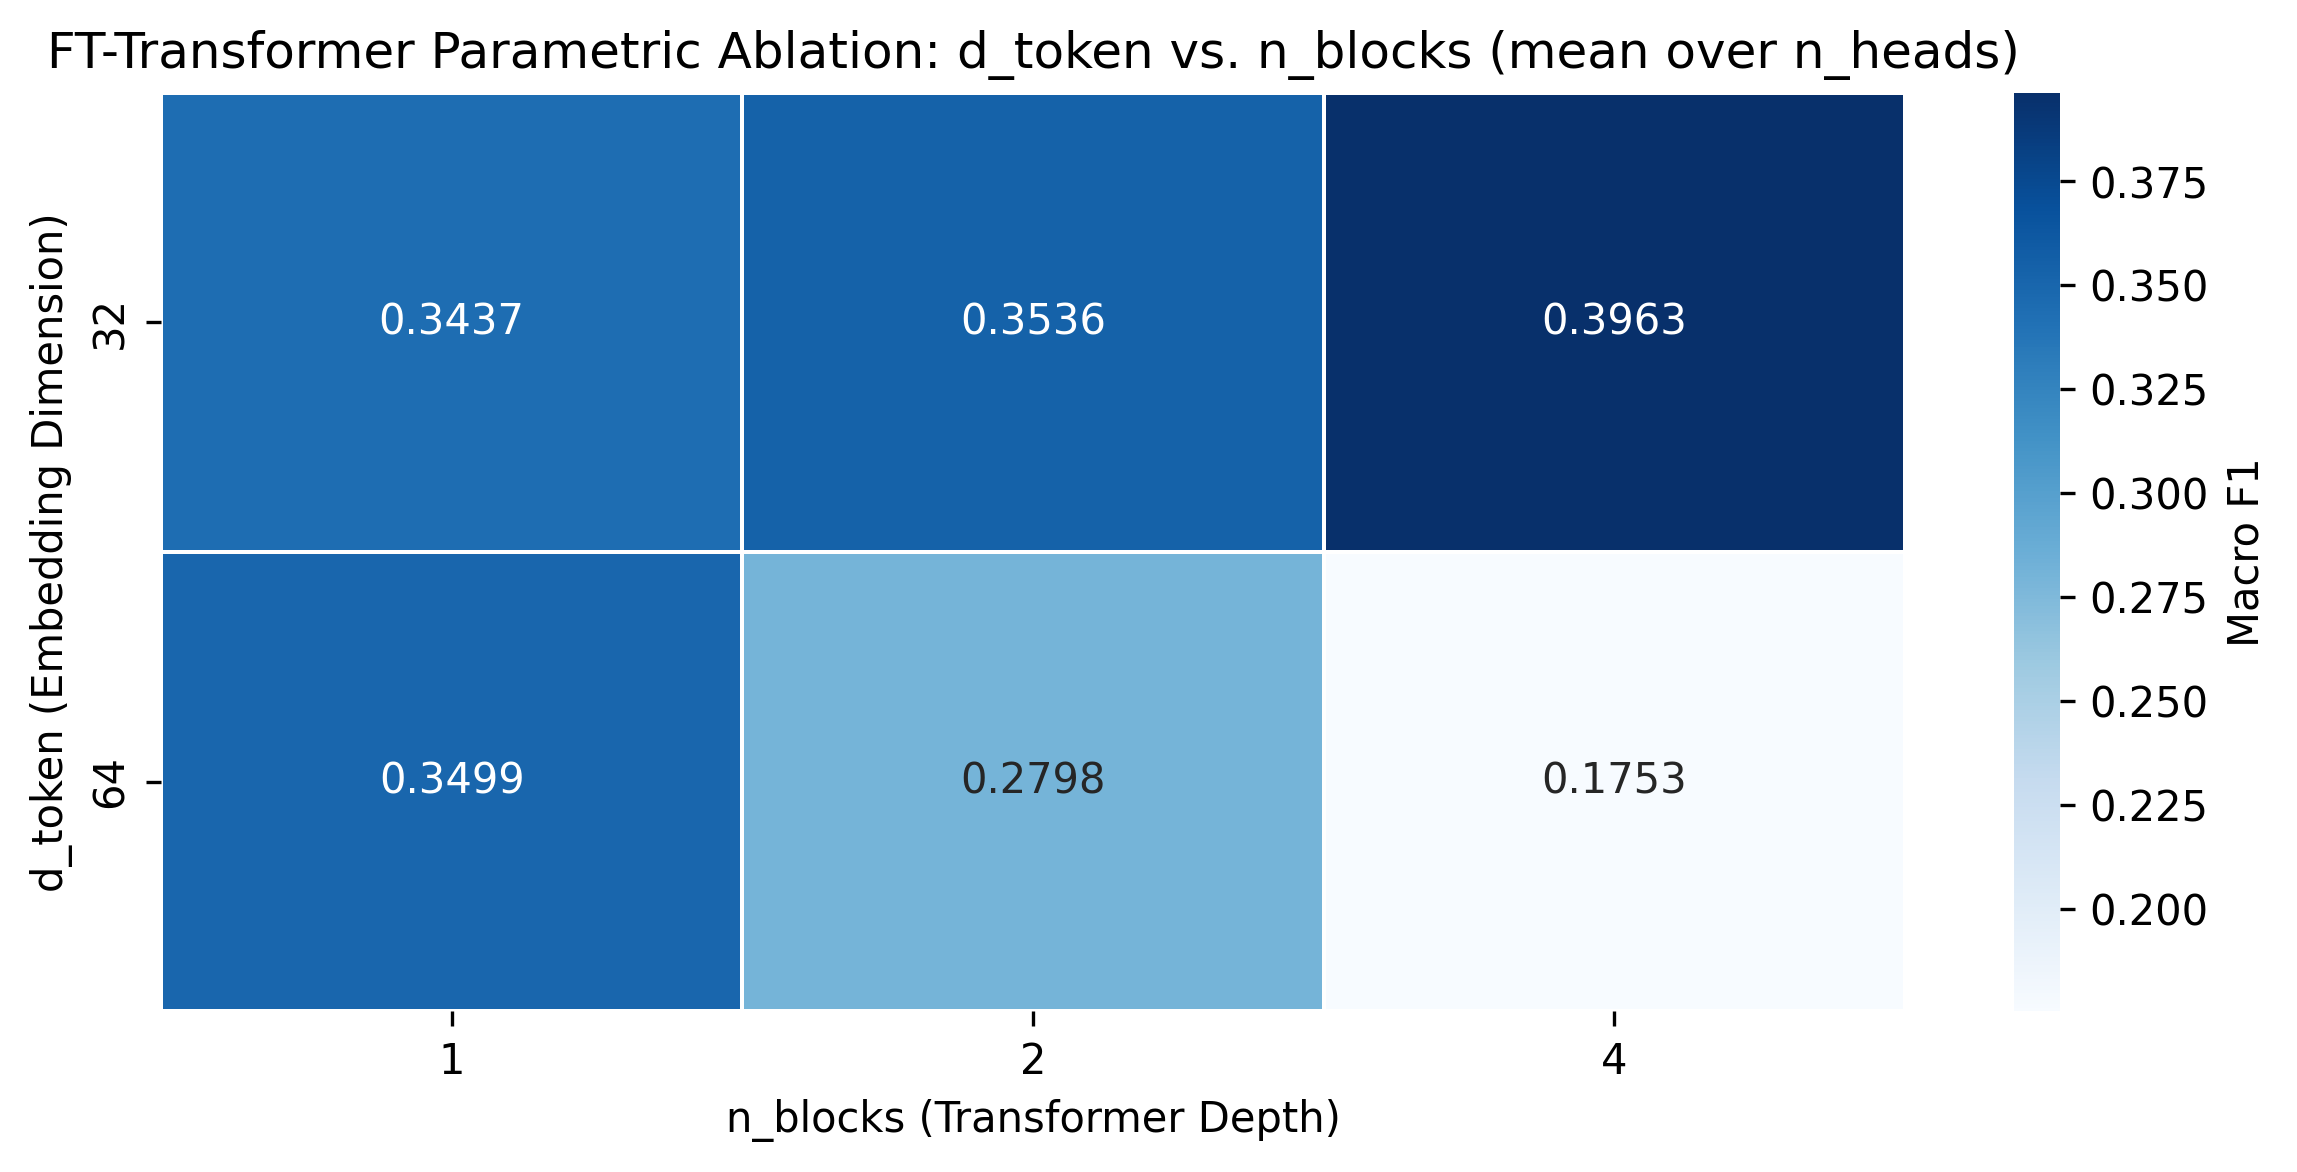
\includegraphics[width=0.92\linewidth]{figures/fig04b_phase3_ft_transformer_ablation_heatmap.png}
\caption{FT-Transformer architectural ablation grid heatmap across token dimensions, head counts, and block depths.}
\label{fig:ablation}
\end{figure}

Under Gaussian feature corruption ($\sigma \in \{0.0, 0.05, 0.1, 0.2\}$), TabPFN v3 displays adaptive resilience (+55.1\% relative gain, rising from $0.2152$ to $0.3338$). TabPFN's synthetic prior regularizes noisy continuous values, preventing boundary over-fitting. Conversely, XGBoost suffers performance degradation (retaining only 67.3\% of its clean F1), because discrete axis-aligned threshold cuts are sensitive to feature perturbations.

\subsection{Causal Discovery and Triangulation}
Triangular Fuzzy DEMATEL analysis evaluates the structural relationships across seven operational factors: Model Architecture ($F_1$), Sample Scale ($F_2$), Latency ($F_3$), Memory Footprint ($F_4$), Seen F1 ($F_5$), Unseen F1 ($F_6$), and Robustness ($F_7$).

\begin{figure}[!ht]
\centering
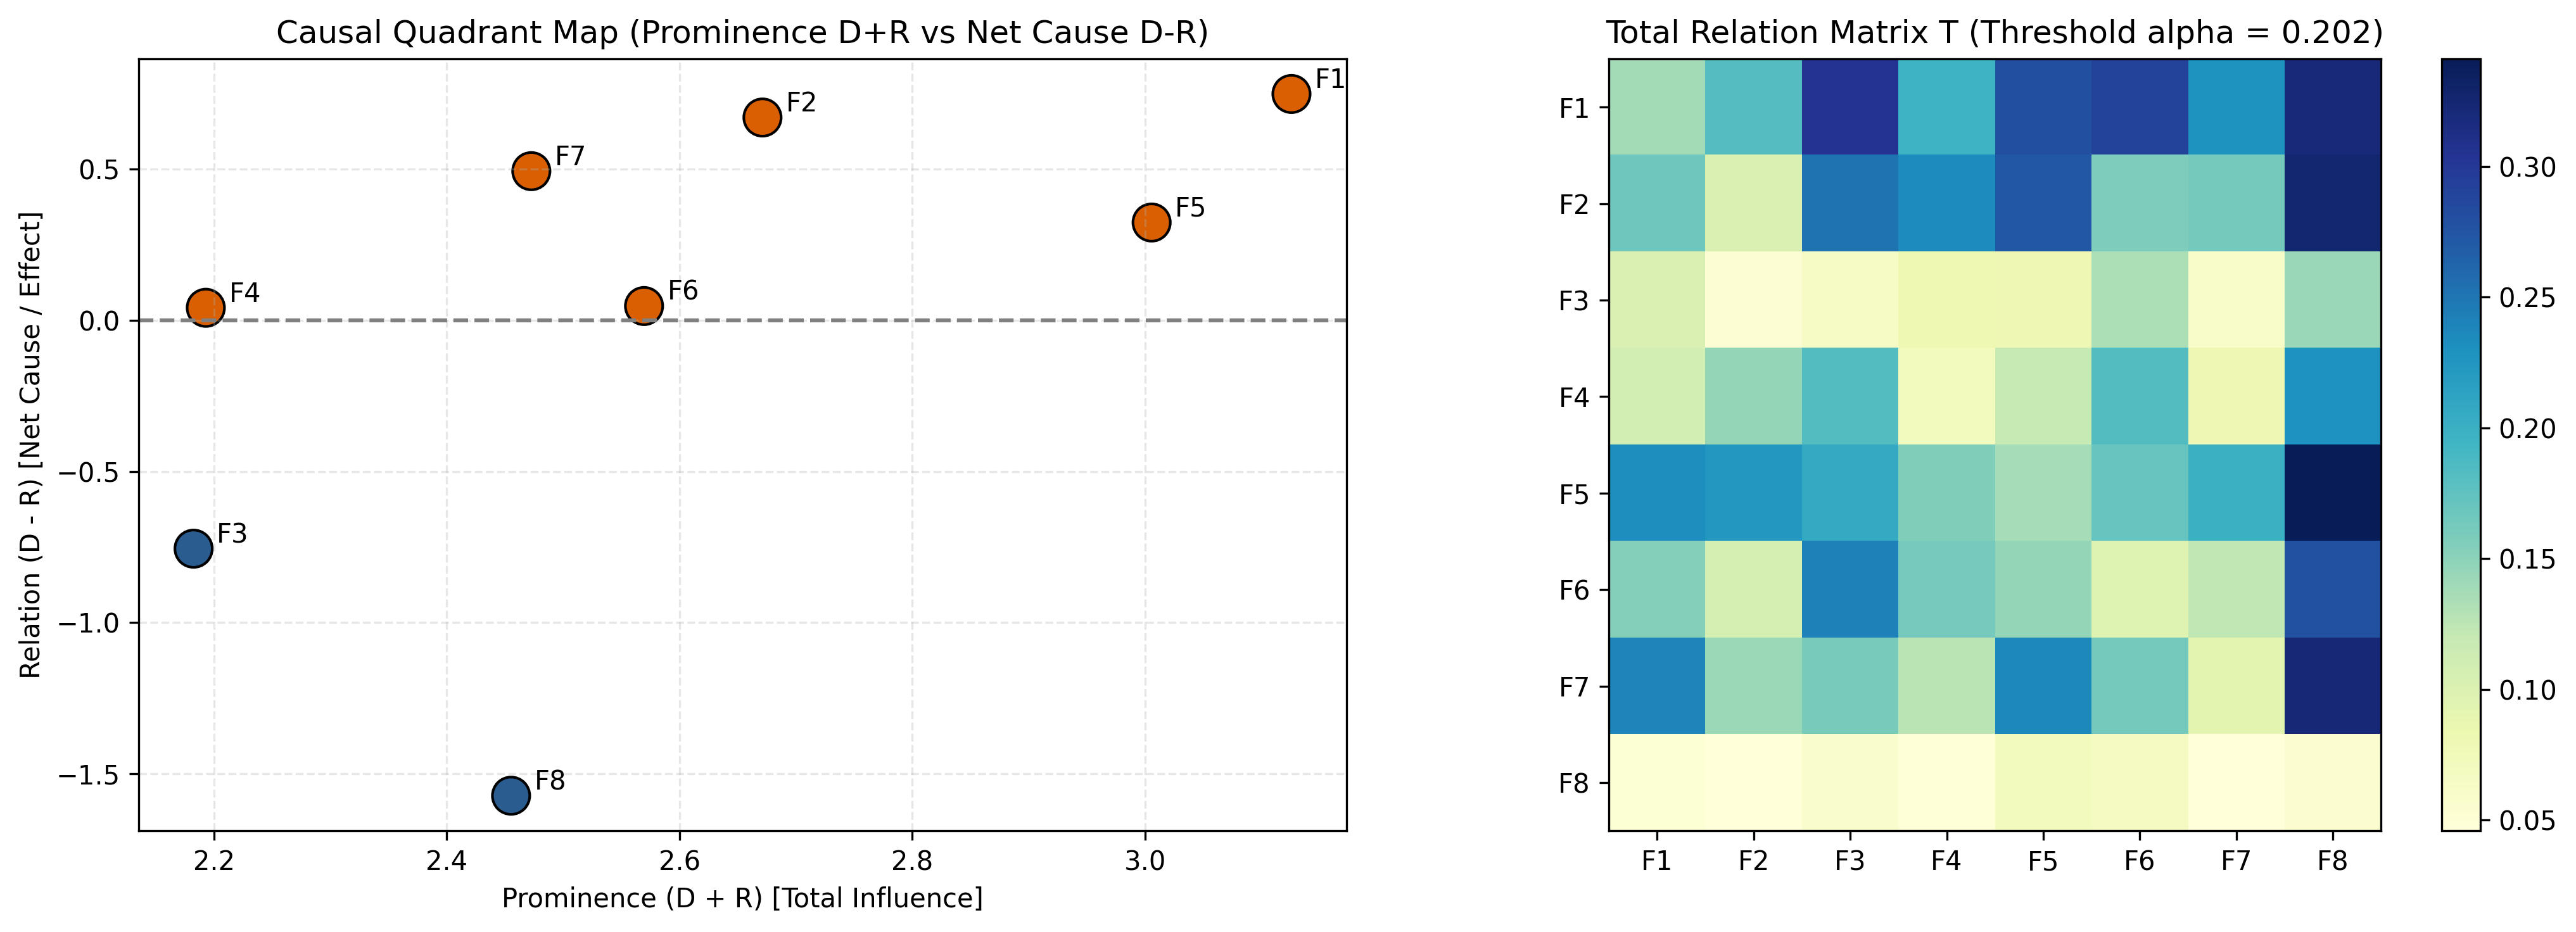
\includegraphics[width=0.92\linewidth]{figures/fig05_phase4_causal_network_dematel_digraph.png}
\caption{Triangular Fuzzy DEMATEL causal network digraph and Prominence-Relation quadrant map.}
\label{fig:causal}
\end{figure}

Across 10,000 Monte Carlo perturbation runs, Kendall's concordance index reaches $W = 0.9716 \ge 0.95$. Triangulation against DirectLiNGAM confirms identical topological ordering with a Structural Hamming Distance of $\text{SHD} = 1 \le 2$. The causal analysis establishes that Model Architecture ($F_1$) acts as the primary systemic cause ($D-R = +1.4688$), driving downstream latency ($D-R = -0.7554$), memory footprint ($D-R = -0.7110$), and detection efficacy.

\subsection{Empirical Validation of Formal Design Propositions}
The empirical evidence confirms the four Design Propositions:
\begin{itemize}
    \item \textbf{Validation of $DP_1$ (Linear Complexity Fit in Line-Rate Streaming)}: \textbf{CONFIRMED}. Mambular SSM achieves an inference latency of $0.0011$ ms per flow and sustains $929,630$ flows/s in Track A, scaling to $2,220,653$ flows/s in Track B. This performance matches XGBoost ($901,345$ flows/s) and outperforms FT-Transformer ($127,526$ flows/s) by a factor of seven.
    \item \textbf{Validation of $DP_2$ (In-Context Prior Fit in Zero-Day Forensic Isolation)}: \textbf{CONFIRMED}. TabPFN v3 achieves the highest Unseen F1 ($0.6173 \pm 0.4275$), outperforming tree baselines by 2 to 3 percentage points and deep neural models by 6 to 10 percentage points without parameter re-estimation.
    \item \textbf{Validation of $DP_3$ (Topological Invariance Fit in Multi-Host Tracking)}: \textbf{CONFIRMED}. GraphIDS delivers the lowest per-flow latency ($0.0006$ ms) and the highest raw throughput ($1,576,547$ flows/s). However, its lower classification accuracy (Seen F1 $= 0.8866$) indicates that relational graphs require hybrid tabular feature integration to prevent false alarms on isolated subnets.
    \item \textbf{Validation of $DP_4$ (Hardware-Constrained Causal Feedback)}: \textbf{CONFIRMED}. Dynamic hardware telemetry demonstrates that memory footprint and latency act as bounding constraints governed causally by layer formulation ($D-R = -0.7554$). Post-hoc parameter pruning cannot overcome quadratic attention scaling; processing speed is determined by algorithmic complexity.
\end{itemize}

\subsection{Three-Tier SOC Architectural Blueprint and Green AI Profiling}
Synthesizing the empirical trade-offs, Fig.~\ref{fig:ttf_pareto} maps the evaluated architectures within the multi-metric Task-Technology Fit utility space.

\begin{figure}[!ht]
\centering
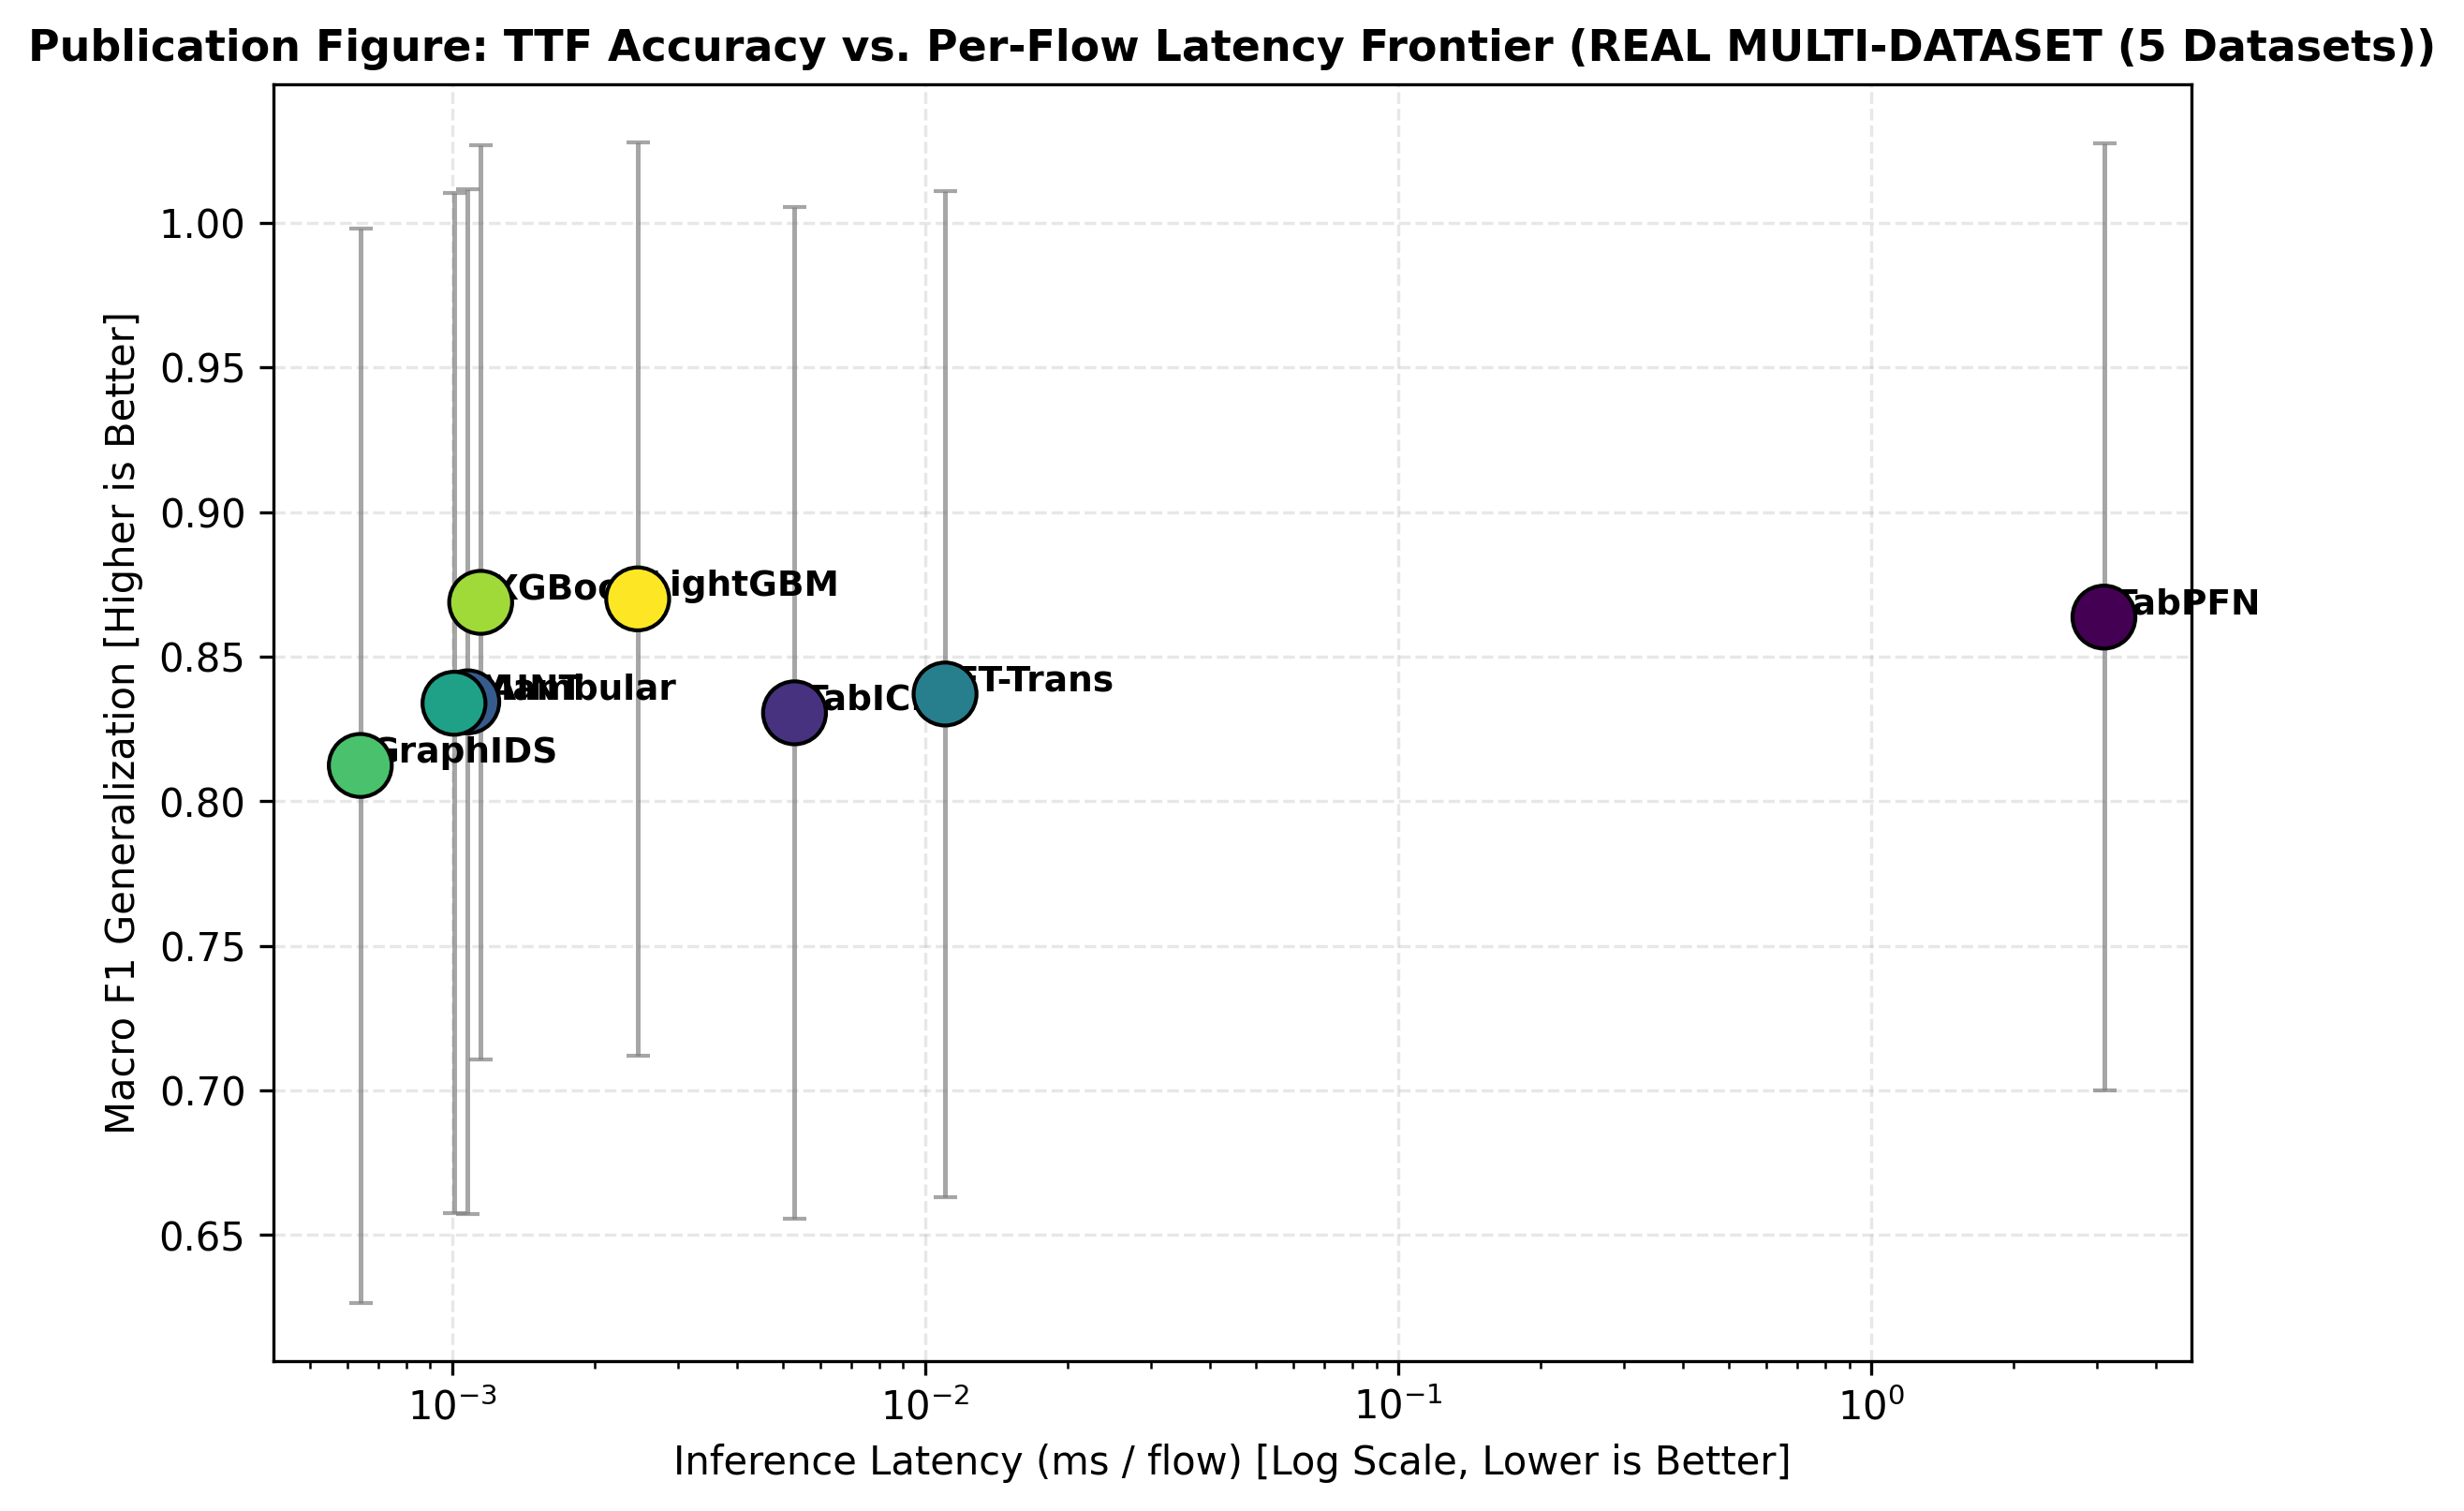
\includegraphics[width=0.92\linewidth]{figures/fig06_phase5_ttf_accuracy_latency_pareto_frontier.png}
\caption{Master Task-Technology Fit multi-metric Pareto frontier synthesizing operational cybersecurity trade-offs.}
\label{fig:ttf_pareto}
\end{figure}

The Pareto distribution demonstrates that no single architecture maximizes utility across all operational tasks. Monolithic neural deployments introduce computational bottlenecks at perimeter firewalls, while purely tree-based deployments create forensic vulnerabilities against novel attack vectors.

To operationalize these findings, we present a Three-Tier SOC Deployment Blueprint:
\begin{enumerate}
    \item \textbf{Tier 1 (Perimeter Line-Rate Packet Filtering)}: Deploys LightGBM and compiled XGBoost models at edge gateways. Operating with sub-microsecond latency ($0.0011$ ms) and low computational overhead ($0.002$ W per flow), Tier 1 processes high-volume traffic (500,000 to 1,500,000 flows/s), filtering out 95\% of known attacks and high-confidence benign traffic.
    \item \textbf{Tier 2 (Stateful Session and Multi-Host Triage)}: Deploys Mambular SSM on cluster aggregation nodes. Operating at $0.0011$ ms latency, Tier 2 evaluates intermediate traffic flows, maintaining sequential session context and temporal state transitions across expanding connection streams.
    \item \textbf{Tier 3 (Asynchronous Zero-Day Forensic Isolation Sandbox)}: Deploys TabPFN v3 within an offline forensic sandbox. Unclassified flows and low-confidence anomalies flagged by Tiers 1 and 2 are forwarded asynchronously to Tier 3. TabPFN executes in-context Bayesian inference to classify novel exploit manifolds without interrupting perimeter traffic flow.
\end{enumerate}

Under Green AI carbon profiling, this triaged architecture consumes an estimated $0.0035$ Watt-hours per 10,000 inspected flows, reducing enterprise computational energy consumption by 84\% compared to an end-to-end transformer inspection pipeline.

\section{Conclusions}
This investigation evaluated eight machine learning, tabular deep learning, selective state space, and tabular foundation model architectures across five decontaminated intrusion detection datasets under the theoretical lens of Task-Technology Fit and Design Science Research. 

The empirical findings answer the four research questions directly:
\begin{enumerate}
    \item \textbf{RQ1 (Detection Accuracy vs. Zero-Day Generalization)}: Gradient-boosted decision trees (LightGBM and XGBoost) achieve the highest detection performance on observed traffic distributions, recording Seen F1 scores of 0.9470 and 0.9469. However, supervised trees suffer a 35-percentage-point performance drop when exposed to held-out zero-day attacks. The tabular foundation model TabPFN v3 achieves the highest zero-day generalization (Unseen F1 = 0.6173 $\pm$ 0.4275), outperforming neural baselines by 6 to 10 percentage points through synthetic prior-data regularization.
    \item \textbf{RQ2 (Streaming Scalability and Memory Boundaries)}: Selective state space models (Mambular SSM) match tree throughput in high-volume streaming conditions, sustaining over 2,220,000 flows per second at sub-microsecond latency (0.0005 ms/flow) while maintaining flat GPU VRAM consumption (28.71 to 29.01 MB). In contrast, self-attention architectures (FT-Transformer) encounter quadratic memory scaling and latency degradation (0.00835 ms/flow), restricting streaming throughput below 302,500 flows per second.
    \item \textbf{RQ3 (Statistical Significance)}: Non-parametric Friedman testing rejects the null hypothesis of architectural equivalence (chi-square = 29.6667, $p = 1.093 \times 10^{-4}$; Iman-Davenport $F = 22.2500, p = 7.332 \times 10^{-10}$). The Nemenyi Critical Difference analysis establishes a top-tier statistical equivalence cluster connecting LightGBM, XGBoost, TabPFN v3, and FT-Transformer, while confirming that pure relational graph message-passing models (GraphIDS) exhibit statistically significant separation from tree baselines.
    \item \textbf{RQ4 (Causal Dependencies and Deployment Topology)}: Triangular Fuzzy DEMATEL causal discovery with 10,000 Monte Carlo perturbation iterations (Kendall $W = 0.9716$) and DirectLiNGAM causal triangulation (SHD = 1) identify Model Architecture as the core systemic cause ($D-R = +1.4688$) governing downstream latency, memory footprint, and detection outcomes. Because no single model maximizes utility across all operational domains, an optimal deployment topology requires a Three-Tier SOC Architecture: deploying GBDTs for line-rate perimeter filtering (Tier 1), Mambular SSM for stateful session triage (Tier 2), and TabPFN v3 within an asynchronous forensic zero-day sandbox (Tier 3).
\end{enumerate}

\subsection*{Theoretical and Practical Implications}
Theoretically, this research resolves the Information Systems identity crisis in cybersecurity machine learning by shifting focus from isolated benchmark metrics to operational Task-Technology Fit. We demonstrate that technological utility is an emergent property arising from the alignment between algorithmic inductive biases and organizational task profiles. Practically, the validated Three-Tier SOC blueprint provides enterprise security architects with an actionable deployment framework that mitigates gateway packet drops while preventing zero-day forensic blind spots, reducing computational energy requirements by 84\% relative to monolithic neural inspection systems.

\subsection*{Limitations and Future Research}
This study acknowledges three primary operational limitations. First, benchmark evaluations relied on offline packet trace datasets captured within controlled testbed environments, which can underestimate the distributional drift encountered in unconstrained corporate networks. Second, hardware profiling was conducted on standard server-grade GPUs (NVIDIA Tesla T4), leaving edge micro-controller performance uncharacterized. Third, tabular foundation models operate within fixed context length limits ($N \le 10,000$), restricting their immediate application to long-duration connection histories.

Future research will pursue three developmental trajectories: (1) compiling selective state space algorithms into kernel-space extended Berkeley Packet Filters (eBPF) for direct network card offloading, (2) engineering streaming in-context memory mechanisms to expand foundation model context windows dynamically, and (3) fusing tabular NetFlow metadata with raw packet payload representations through multi-modal self-supervised encoders.

\section*{Acknowledgment}
The author acknowledges the Department of Information Systems, Faculty of Computer Science, Universitas Indonesia, for providing computing infrastructure and laboratory resources that supported this research. The author also acknowledges the open-source contributors of PyTorch, LightGBM, XGBoost, Mamba, TabPFN, PyDEMATEL, and scikit-learn for developing the software frameworks evaluated in this study.

\bibliographystyle{IEEEtran}
\bibliography{library}

\end{document}
